
%% bare_jrnl.tex
%% V1.4b
%% 2015/08/26
%% by Michael Shell
%% see http://www.michaelshell.org/
%% for current contact information.
%%
%% This is a skeleton file demonstrating the use of IEEEtran.cls
%% (requires IEEEtran.cls version 1.8b or later) with an IEEE
%% journal paper.
%%
%% Support sites:
%% http://www.michaelshell.org/tex/ieeetran/
%% http://www.ctan.org/pkg/ieeetran
%% and
%% http://www.ieee.org/

%%*************************************************************************
%% Legal Notice:
%% This code is offered as-is without any warranty either expressed or
%% implied; without even the implied warranty of MERCHANTABILITY or
%% FITNESS FOR A PARTICULAR PURPOSE! 
%% User assumes all risk.
%% In no event shall the IEEE or any contributor to this code be liable for
%% any damages or losses, including, but not limited to, incidental,
%% consequential, or any other damages, resulting from the use or misuse
%% of any information contained here.
%%
%% All comments are the opinions of their respective authors and are not
%% necessarily endorsed by the IEEE.
%%
%% This work is distributed under the LaTeX Project Public License (LPPL)
%% ( http://www.latex-project.org/ ) version 1.3, and may be freely used,
%% distributed and modified. A copy of the LPPL, version 1.3, is included
%% in the base LaTeX documentation of all distributions of LaTeX released
%% 2003/12/01 or later.
%% Retain all contribution notices and credits.
%% ** Modified files should be clearly indicated as such, including  **
%% ** renaming them and changing author support contact information. **
%%*************************************************************************


% *** Authors should verify (and, if needed, correct) their LaTeX system  ***
% *** with the testflow diagnostic prior to trusting their LaTeX platform ***
% *** with production work. The IEEE's font choices and paper sizes can   ***
% *** trigger bugs that do not appear when using other class files.       ***                          ***
% The testflow support page is at:
% http://www.michaelshell.org/tex/testflow/



\documentclass[journal]{IEEEtran}
%
% If IEEEtran.cls has not been installed into the LaTeX system files,
% manually specify the path to it like:
% \documentclass[journal]{../sty/IEEEtran}





% Some very useful LaTeX packages include:
% (uncomment the ones you want to load)


% *** MISC UTILITY PACKAGES ***
%
%\usepackage{ifpdf}
% Heiko Oberdiek's ifpdf.sty is very useful if you need conditional
% compilation based on whether the output is pdf or dvi.
% usage:
% \ifpdf
%   % pdf code
% \else
%   % dvi code
% \fi
% The latest version of ifpdf.sty can be obtained from:
% http://www.ctan.org/pkg/ifpdf
% Also, note that IEEEtran.cls V1.7 and later provides a builtin
% \ifCLASSINFOpdf conditional that works the same way.
% When switching from latex to pdflatex and vice-versa, the compiler may
% have to be run twice to clear warning/error messages.






% *** CITATION PACKAGES ***
%
\usepackage{cite}
% cite.sty was written by Donald Arseneau
% V1.6 and later of IEEEtran pre-defines the format of the cite.sty package
% \cite{} output to follow that of the IEEE. Loading the cite package will
% result in citation numbers being automatically sorted and properly
% "compressed/ranged". e.g., [1], [9], [2], [7], [5], [6] without using
% cite.sty will become [1], [2], [5]--[7], [9] using cite.sty. cite.sty's
% \cite will automatically add leading space, if needed. Use cite.sty's
% noadjust option (cite.sty V3.8 and later) if you want to turn this off
% such as if a citation ever needs to be enclosed in parenthesis.
% cite.sty is already installed on most LaTeX systems. Be sure and use
% version 5.0 (2009-03-20) and later if using hyperref.sty.
% The latest version can be obtained at:
% http://www.ctan.org/pkg/cite
% The documentation is contained in the cite.sty file itself.






% *** GRAPHICS RELATED PACKAGES ***
%
\ifCLASSINFOpdf
  \usepackage[pdftex]{graphicx}
  % declare the path(s) where your graphic files are
  \graphicspath{{./pics/}}
  % and their extensions so you won't have to specify these with
  % every instance of \includegraphics
  \DeclareGraphicsExtensions{.pdf,.jpeg,.png}
\else
  % or other class option (dvipsone, dvipdf, if not using dvips). graphicx
  % will default to the driver specified in the system graphics.cfg if no
  % driver is specified.
  \usepackage[dvips]{graphicx}
  % declare the path(s) where your graphic files are
  \graphicspath{{./pics/}}
  % and their extensions so you won't have to specify these with
  % every instance of \includegraphics
  \DeclareGraphicsExtensions{.eps}
\fi
% graphicx was written by David Carlisle and Sebastian Rahtz. It is
% required if you want graphics, photos, etc. graphicx.sty is already
% installed on most LaTeX systems. The latest version and documentation
% can be obtained at: 
% http://www.ctan.org/pkg/graphicx
% Another good source of documentation is "Using Imported Graphics in
% LaTeX2e" by Keith Reckdahl which can be found at:
% http://www.ctan.org/pkg/epslatex
%
% latex, and pdflatex in dvi mode, support graphics in encapsulated
% postscript (.eps) format. pdflatex in pdf mode supports graphics
% in .pdf, .jpeg, .png and .mps (metapost) formats. Users should ensure
% that all non-photo figures use a vector format (.eps, .pdf, .mps) and
% not a bitmapped formats (.jpeg, .png). The IEEE frowns on bitmapped formats
% which can result in "jaggedy"/blurry rendering of lines and letters as
% well as large increases in file sizes.
%
% You can find documentation about the pdfTeX application at:
% http://www.tug.org/applications/pdftex





% *** MATH PACKAGES ***
%
\usepackage{amsmath,amsthm}
% A popular package from the American Mathematical Society that provides
% many useful and powerful commands for dealing with mathematics.
%
% Note that the amsmath package sets \interdisplaylinepenalty to 10000
% thus preventing page breaks from occurring within multiline equations. Use:
%\interdisplaylinepenalty=2500
% after loading amsmath to restore such page breaks as IEEEtran.cls normally
% does. amsmath.sty is already installed on most LaTeX systems. The latest
% version and documentation can be obtained at:
% http://www.ctan.org/pkg/amsmath





% *** SPECIALIZED LIST PACKAGES ***
%
%\usepackage{algorithmic}
% algorithmic.sty was written by Peter Williams and Rogerio Brito.
% This package provides an algorithmic environment fo describing algorithms.
% You can use the algorithmic environment in-text or within a figure
% environment to provide for a floating algorithm. Do NOT use the algorithm
% floating environment provided by algorithm.sty (by the same authors) or
% algorithm2e.sty (by Christophe Fiorio) as the IEEE does not use dedicated
% algorithm float types and packages that provide these will not provide
% correct IEEE style captions. The latest version and documentation of
% algorithmic.sty can be obtained at:
% http://www.ctan.org/pkg/algorithms
% Also of interest may be the (relatively newer and more customizable)
% algorithmicx.sty package by Szasz Janos:
% http://www.ctan.org/pkg/algorithmicx




% *** ALIGNMENT PACKAGES ***
%
%\usepackage{array}
% Frank Mittelbach's and David Carlisle's array.sty patches and improves
% the standard LaTeX2e array and tabular environments to provide better
% appearance and additional user controls. As the default LaTeX2e table
% generation code is lacking to the point of almost being broken with
% respect to the quality of the end results, all users are strongly
% advised to use an enhanced (at the very least that provided by array.sty)
% set of table tools. array.sty is already installed on most systems. The
% latest version and documentation can be obtained at:
% http://www.ctan.org/pkg/array


% IEEEtran contains the IEEEeqnarray family of commands that can be used to
% generate multiline equations as well as matrices, tables, etc., of high
% quality.




% *** SUBFIGURE PACKAGES ***
%\ifCLASSOPTIONcompsoc
%  \usepackage[caption=false,font=normalsize,labelfont=sf,textfont=sf]{subfig}
%\else
\usepackage[caption=false,font=footnotesize]{subfig}
%\fi
% subfig.sty, written by Steven Douglas Cochran, is the modern replacement
% for subfigure.sty, the latter of which is no longer maintained and is
% incompatible with some LaTeX packages including fixltx2e. However,
% subfig.sty requires and automatically loads Axel Sommerfeldt's caption.sty
% which will override IEEEtran.cls' handling of captions and this will result
% in non-IEEE style figure/table captions. To prevent this problem, be sure
% and invoke subfig.sty's "caption=false" package option (available since
% subfig.sty version 1.3, 2005/06/28) as this is will preserve IEEEtran.cls
% handling of captions.
% Note that the Computer Society format requires a larger sans serif font
% than the serif footnote size font used in traditional IEEE formatting
% and thus the need to invoke different subfig.sty package options depending
% on whether compsoc mode has been enabled.
%
% The latest version and documentation of subfig.sty can be obtained at:
% http://www.ctan.org/pkg/subfig




% *** FLOAT PACKAGES ***
%
%\usepackage{fixltx2e}
% fixltx2e, the successor to the earlier fix2col.sty, was written by
% Frank Mittelbach and David Carlisle. This package corrects a few problems
% in the LaTeX2e kernel, the most notable of which is that in current
% LaTeX2e releases, the ordering of single and double column floats is not
% guaranteed to be preserved. Thus, an unpatched LaTeX2e can allow a
% single column figure to be placed prior to an earlier double column
% figure.
% Be aware that LaTeX2e kernels dated 2015 and later have fixltx2e.sty's
% corrections already built into the system in which case a warning will
% be issued if an attempt is made to load fixltx2e.sty as it is no longer
% needed.
% The latest version and documentation can be found at:
% http://www.ctan.org/pkg/fixltx2e


%\usepackage{stfloats}
% stfloats.sty was written by Sigitas Tolusis. This package gives LaTeX2e
% the ability to do double column floats at the bottom of the page as well
% as the top. (e.g., "\begin{figure*}[!b]" is not normally possible in
% LaTeX2e). It also provides a command:
%\fnbelowfloat
% to enable the placement of footnotes below bottom floats (the standard
% LaTeX2e kernel puts them above bottom floats). This is an invasive package
% which rewrites many portions of the LaTeX2e float routines. It may not work
% with other packages that modify the LaTeX2e float routines. The latest
% version and documentation can be obtained at:
% http://www.ctan.org/pkg/stfloats
% Do not use the stfloats baselinefloat ability as the IEEE does not allow
% \baselineskip to stretch. Authors submitting work to the IEEE should note
% that the IEEE rarely uses double column equations and that authors should try
% to avoid such use. Do not be tempted to use the cuted.sty or midfloat.sty
% packages (also by Sigitas Tolusis) as the IEEE does not format its papers in
% such ways.
% Do not attempt to use stfloats with fixltx2e as they are incompatible.
% Instead, use Morten Hogholm'a dblfloatfix which combines the features
% of both fixltx2e and stfloats:
%
% \usepackage{dblfloatfix}
% The latest version can be found at:
% http://www.ctan.org/pkg/dblfloatfix




%\ifCLASSOPTIONcaptionsoff
%  \usepackage[nomarkers]{endfloat}
% \let\MYoriglatexcaption\caption
% \renewcommand{\caption}[2][\relax]{\MYoriglatexcaption[#2]{#2}}
%\fi
% endfloat.sty was written by James Darrell McCauley, Jeff Goldberg and 
% Axel Sommerfeldt. This package may be useful when used in conjunction with 
% IEEEtran.cls'  captionsoff option. Some IEEE journals/societies require that
% submissions have lists of figures/tables at the end of the paper and that
% figures/tables without any captions are placed on a page by themselves at
% the end of the document. If needed, the draftcls IEEEtran class option or
% \CLASSINPUTbaselinestretch interface can be used to increase the line
% spacing as well. Be sure and use the nomarkers option of endfloat to
% prevent endfloat from "marking" where the figures would have been placed
% in the text. The two hack lines of code above are a slight modification of
% that suggested by in the endfloat docs (section 8.4.1) to ensure that
% the full captions always appear in the list of figures/tables - even if
% the user used the short optional argument of \caption[]{}.
% IEEE papers do not typically make use of \caption[]'s optional argument,
% so this should not be an issue. A similar trick can be used to disable
% captions of packages such as subfig.sty that lack options to turn off
% the subcaptions:
% For subfig.sty:
% \let\MYorigsubfloat\subfloat
% \renewcommand{\subfloat}[2][\relax]{\MYorigsubfloat[]{#2}}
% However, the above trick will not work if both optional arguments of
% the \subfloat command are used. Furthermore, there needs to be a
% description of each subfigure *somewhere* and endfloat does not add
% subfigure captions to its list of figures. Thus, the best approach is to
% avoid the use of subfigure captions (many IEEE journals avoid them anyway)
% and instead reference/explain all the subfigures within the main caption.
% The latest version of endfloat.sty and its documentation can obtained at:
% http://www.ctan.org/pkg/endfloat
%
% The IEEEtran \ifCLASSOPTIONcaptionsoff conditional can also be used
% later in the document, say, to conditionally put the References on a 
% page by themselves.




% *** PDF, URL AND HYPERLINK PACKAGES ***
%
%\usepackage{url}
% url.sty was written by Donald Arseneau. It provides better support for
% handling and breaking URLs. url.sty is already installed on most LaTeX
% systems. The latest version and documentation can be obtained at:
% http://www.ctan.org/pkg/url
% Basically, \url{my_url_here}.




% *** Do not adjust lengths that control margins, column widths, etc. ***
% *** Do not use packages that alter fonts (such as pslatex).         ***
% There should be no need to do such things with IEEEtran.cls V1.6 and later.
% (Unless specifically asked to do so by the journal or conference you plan
% to submit to, of course. )


% correct bad hyphenation here
\hyphenation{op-tical net-works semi-conduc-tor}

\usepackage{color}
\usepackage{amsfonts,amssymb}
\usepackage{soul}

\newtheorem{theorem}{Theorem}[section]
\newtheorem{corollary}{Corollary}[section]
\newtheorem{remark}{Remark}[section]
\newtheorem{lemma}{Lemma}[section]

\newcommand{\mauricio}[1]{{\color{blue}#1}}

\newcommand{\simo}[1]{{\color{red}#1}}

\begin{document}
%
% paper title
% can use linebreaks \\ within to get better formatting as desired
% Do not put math or special symbols in the title.
%\title{Latent force models for signal processing and machine learning }
%\title{Combining First-Principles and Non-Parametric Statistical Models via Latent Force Models}
\title{Gaussian Process Latent Force Models for Learning and Stochastic Control of Physical Systems}


%
%
% author names and IEEE memberships
% note positions of commas and nonbreaking spaces ( ~ ) LaTeX will not break
% a structure at a ~ so this keeps an author's name from being broken across
% two lines.
% use \thanks{} to gain access to the first footnote area
% a separate \thanks must be used for each paragraph as LaTeX2e's \thanks
% was not built to handle multiple paragraphs
%

\author{Simo~S\"arkk\"a,~\IEEEmembership{Senior Member,~IEEE,}
        Mauricio~A.~\'Alvarez, 
        and~Neil~D.~Lawrence% <-this % stops a space
\thanks{Simo~S\"arkk\"a is with the Department of Electrical Engineering and Automation (EEA), Aalto University, Rakentajanaukio 2, 02150 Espoo, Finland (simo.sarkka@aalto.fi).}% <-this % stops a space
\thanks{Mauricio A. \'Alvarez is with the Department of Computer Science, University of Sheffield,
Sheffield, UK S1 4DP}% <-this % stops a space
\thanks{Neil D. Lawrence is with Amazon, Cambridge, UK and the Department of Computer Science, University of Sheffield,
Sheffield, UK S1 4DP}% <-this % stops a space
\thanks{Manuscript received XXX; revised XXX.}}


% note the % following the last \IEEEmembership and also \thanks -
% these prevent an unwanted space from occurring between the last author name
% and the end of the author line. i.e., if you had this:
%
% \author{....lastname \thanks{...} \thanks{...} }
%                     ^------------^------------^----Do not want these spaces!
%
% a space would be appended to the last name and could cause every name on that
% line to be shifted left slightly. This is one of those "LaTeX things". For
% instance, "\textbf{A} \textbf{B}" will typeset as "A B" not "AB". To get
% "AB" then you have to do: "\textbf{A}\textbf{B}"
% \thanks is no different in this regard, so shield the last } of each \thanks
% that ends a line with a % and do not let a space in before the next \thanks.
% Spaces after \IEEEmembership other than the last one are OK (and needed) as
% you are supposed to have spaces between the names. For what it is worth,
% this is a minor point as most people would not even notice if the said evil
% space somehow managed to creep in.



% The paper headers
\markboth{Journal of \LaTeX\ Class Files,~Vol.~X, No.~X, Month~20XX}%
{Shell \MakeLowercase{\textit{et al.}}: Bare Demo of IEEEtran.cls for Journals}
% The only time the second header will appear is for the odd numbered pages
% after the title page when using the twoside option.
%
% *** Note that you probably will NOT want to include the author's ***
% *** name in the headers of peer review papers.                   ***
% You can use \ifCLASSOPTIONpeerreview for conditional compilation here if
% you desire.




% If you want to put a publisher's ID mark on the page you can do it like
% this:
%\IEEEpubid{0000--0000/00\$00.00~\copyright~2012 IEEE}
% Remember, if you use this you must call \IEEEpubidadjcol in the second
% column for its text to clear the IEEEpubid mark.



% use for special paper notices
%\IEEEspecialpapernotice{(Invited Paper)}




% make the title area
\maketitle

% As a general rule, do not put math, special symbols or citations
% in the abstract or keywords.
\begin{abstract}
This paper is concerned with estimation and stochastic control in physical systems which contain unknown input signals or forces. These unknown signals are modeled as Gaussian processes (GP) in the sense that GP models are used in machine learning. The resulting  latent force models (LFMs) can be seen as hybrid models that contain a first-principles physical model part and a non-parametric GP model part. The aim of this paper is to collect and extend the statistical inference and learning methods for this kind of models, provide new theoretical results for the models, and to extend the methodology and theory to stochastic control of LFMs. 
\end{abstract}

% Note that keywords are not normally used for peerreview papers.
\begin{IEEEkeywords}
Gaussian process, latent force model, stochastic control, statistical learning, statistical inference.
\end{IEEEkeywords}



% For peer review papers, you can put extra information on the cover
% page as needed:
% \ifCLASSOPTIONpeerreview
% \begin{center} \bfseries EDICS Category: 3-BBND \end{center}
% \fi
%
% For peerreview papers, this IEEEtran command inserts a page break and
% creates the second title. It will be ignored for other modes.
\IEEEpeerreviewmaketitle



\section{Introduction}
%\simo{We need to revise the following -- let's not tell here what people in machine learning are interested, but instead tell why LFMs would save the world in this field. This text is also too chatty, this can be cut to half. However, we need to have a short introduction Gaussian process regression here.}

%\IEEEPARstart{I}{n} machine learning, there has been a recent interest to combine non-parametric statistical models with first-principles physical differential equation models. The motivation to do that is that although non-parametric statistical models such as Gaussian processes \cite{Rasmussen+Williams:2006} are well-suited for expressing very loose assumptions on the modeled functions (such as smoothness and length scale), encoding physical knowledge into them is hard. In many applications, we are faced with problems in which we have plenty of data and a physical model, and we want to use statistical inference either to estimate the parameters of those physical models or to perform inference over unknown functions or variables related to the physical model. This setup appears frequently in modern physics, biology, chemistry, geology, and many other scientific disciplines for which the description of physical phenomena is done through differential equations. To deal with these kinds of problems, we recently introduced latent force models (LFM) \cite{Alvarez+Lawrence:2009,Alvarez:2010,Alvarez+Luengo+Lawrence:2013}, which are general models that allow the incorporation of differential equations into data-driven non-parametric models -- or non-parametric models into differential equation models.

%\simo{{\em Notation:} $n$ is the number of data points, $p$ is the input ($\mathbf{x}$) dimension, $d$ is the vector output dimensionality, $s$ for order of ODE or state-space or half-order of spectral density denominator (these are the same things), $r$ for the half-order of spectral density numerator, $k$ is the discrete time index, if we have space and time, $n = n_x \, n_t$ for data points in time and space (for a grid). Todo: check the operator fonts.}

\IEEEPARstart{C}{onsider}, as an example, a second order differential equation model of a physical system of the form
%
\begin{equation}
\begin{split}
  \frac{d^{2}f(t)}{dt^{2}} + \lambda \, \frac{df(t)}{dt} + \gamma \, f(t) = u(t) + c(t),
\end{split}
\label{eq:sde0}
\end{equation}
%
where the functions $u(t)$ and $f(t)$ are unknown an $c(t)$ is a control function (known or to be optimized). Further assume that we measure the function $f(t)$ via noisy measurements at discrete instants of time $t_1,t_2,\ldots$:
%
\begin{equation}
\begin{split}
  y_k &= f(t_k) + \epsilon_k,
\end{split}
\end{equation}
%
The aim of this article is to consider the unknown force or input $u$ as unknown and model it as a non-parametric Gaussian process model \cite{Rasmussen+Williams:2006} with a given covariance function in order to estimate, or in machine learning terms, {\em learn} $f$ and $u$. The generalizations of this kind of models to arbitrary differential equations are called latent force models (LFM) \cite{Alvarez+Luengo+Lawrence:2009,Alvarez:2010,Alvarez+Luengo+Lawrence:2013,Hartikainen+Sarkka:2011,Hartikainen+Seppanen+Sarkka:2012} in machine learning literature. In addition to learning problem on the LFMs, we also consider the problem of controlling the LFM using the control function $c(t)$. In particular, we consider the problem of optimal stochastic control design for LFMs.

The present problem is also closely related to so called input estimation problem that has previously been addressed in target tracking literature (e.g. \cite{Bar-Shalom+Li+Kirubarajan:2001}) by replacing the input or force with a white or colored noise. However, here we will specifically concentrate on the machine learning point of view which allows for encoding prior information into the driving force as well as the use of modern machine learning methods for coping with the related hyperparameter estimation problems and model extensions. 

In addition to \eqref{eq:sde0}, other examples of problems of interest are spatio-temporal partial differential equations driven by (structured) Gaussian processes such as the controlled heat equation
%
\begin{equation}
\begin{split}
  \frac{\partial f(\mathbf{x},t)}{\partial t} &=
  D \, \nabla^2 \, f(\mathbf{x},t) - \beta \, f(\mathbf{x},t) \\
  &\qquad + u(\mathbf{x},t) + c(\mathbf{x},t) \\
  y_k &= f(\mathbf{x}_k,t_k) + \epsilon_k,
\end{split}
\label{eq:spde0}
\end{equation}
%
where again the aim is to learn both the Gaussian force field $u(\mathbf{x},t)$ and the function $f(\mathbf{x},t)$ from
the noisy observations $y_k$ as well as design an optimal control for \mauricio{regulating the heat. should we define D
  and beta in the heat equation?}

%In both temporal models \eqref{eq:sde0} and spatio-temporal models \eqref{eq:spde0} we also consider the associated stochastic control problem: how can we simultaneously learn the functions $f$ and $u$, and design an optimal stochastic controller $c$ which uses the learning outcome optimally. It turns out that this problem can be recasted as a classical stochastic control problem (e.g., \cite{Maybeck:1982b}) in an augmented state-space provided that we convert the Gaussian process input model into an equivalent stochastic state-space representation \cite{Hartikainen+Sarkka:2010,Hartikainen+Sarkka:2011,Hartikainen+Seppanen+Sarkka:2012}.

A different kind of example of a problem studied in this article is the Poisson equation
%
\begin{equation}
\begin{split}
  \nabla^2 f(\mathbf{x}) &= u(\mathbf{x}) \\
  y_k &= f(\mathbf{x}_k) + \epsilon_k,
\end{split}
\label{eq:poisson0}
\end{equation}
%
where again the function $f$ and the force field $u$ are unknown. The difference is that here is no concept of time in this equation, nor a possibility for controlling the equation. However, the problem of estimating the function $f$ and the force field $u$ from the observations $y_k$ is still well defined.


%LFMs can be derived from two different perspectives: the covariance function perspective \cite{Alvarez+Lawrence:2009,Alvarez+Luengo+Lawrence:2013} and the state-space perspective \cite{Hartikainen+Sarkka:2011,Hartikainen+Seppanen+Sarkka:2012}. The former approach can be seen as a machine learning point of view (cf. \cite{Rasmussen+Williams:2006}) to LFMs whereas the latter approach is a signal processing point of view (cf. \cite{Sarkka+Solin+Hartikainen:2013,Sarkka:2013}). Both of these approaches have their own advantages and disadvantages in terms of flexibility, ease of implementation, and computational complexity. In this paper, we analyze both of these points of view to latent force models as well as present new computational methods which aim to combine the best sides of both points of view. 

% \simo{Explain here what has been done before and what is actually new here.}

%The new contributions of this article are:
%%
%\begin{itemize}
%\item \simo{Unified treatment of batch and state space.}
%\item \simo{Particle differential equation methods.}
%\item \simo{Control problems.}
%\item \simo{Detectability and stabilizability.}
%\end{itemize}

\subsection{General problem formulation}
%
The models considered in this article can be seen to belong to the following three classes:
%
\begin{enumerate}
\item Basic latent force models which are ordinary differential equations (ODEs) driven by Gaussian input processes $u(t)$ and control inputs $c(t)$. They can be written in form
%
\begin{equation}
  \mathcal{L} \, f(t) = u(t) + c(t),
\label{eq:Lfuc1}
\end{equation}
%
where the linear operator is typically $\mathcal{L}\equiv a_n \, \frac{d}{dt^{n}} + \cdots + a_1 \, \frac{d}{dt} + a_0$ for some fixed constants $a_i, i=0,\ldots,n$. This kind of models can often be rewritten in 
\emph{state-space form}
%
\begin{equation}
  \frac{d\mathbf{f}(t)}{dt} = \mathbf{A}_f \, \mathbf{f}(t) + \mathbf{B}_f \, \mathbf{u}(t) + \mathbf{M}_f \, \mathbf{c}(t),
\end{equation}
%
which is not only equivalent to the representation above, but strictly more general model formulation that \eqref{eq:Lfuc1}; the control $\mathbf{c}$ can be a vector and it does not need to enter the system via the same route as the latent force, and the operator $\mathcal{L}$ can also be an integro-differential operator.

\item We also consider are dynamic partial and pseudo differential equation (PDE) based models that can generally be written in form
%
\begin{equation}
  \mathcal{L} \, f(\mathbf{x},t) = u(\mathbf{x},t) + c(\mathbf{x},t),
\label{eq:Lfuc2}
\end{equation}
%
where $\mathcal{L}$ is a linear operator in space and time. The input Gaussian process $u(\mathbf{x},t)$ and control input $c(\mathbf{x},t)$ are also space-time processes. Typically, the operator as the form
%
\begin{equation}
  \mathcal{L}\equiv \mathcal{A}_n \, \frac{d}{dt^{n}} + \cdots + \mathcal{A}_1 \, \frac{d}{dt} + \mathcal{A}_0,
\label{eq:Lfuc2}
\end{equation}
%
where $\mathcal{A}_0,\ldots,\mathcal{A}_n$ are some spatial partial differential or pseudo-differential operators. This kind of models can often be also written in form of \emph{spatio-temporal state-space models}
%
\begin{equation}
\begin{split}
  \frac{\partial \mathbf{f}(\mathbf{x},t)}{\partial t}
  &= \mathbf{\mathcal{A}}_f \, \mathbf{f}(\mathbf{x},t) + \mathbf{B}_f \, u(\mathbf{x},t) + \mathbf{M}_f \, \mathbf{c}(\mathbf{x},t),
\end{split}
\end{equation}
%
which again is strictly more general than the model \eqref{eq:Lfuc2}. 

\item As a static special case of the above models we have the following class of partial and pseudo differential equation (PDE) models driven by spatial Gaussian processes $u(\mathbf{x})$:
%
\begin{equation}
  \mathcal{L} \, f(\mathbf{x}) = u(\mathbf{x}),
\end{equation}
%
where $\mathcal{L}$ is a spatial partial differential operator or pseudo-differential operator. For this kind of models there is no control problem per se, because there is no time dependence.  These models do not naturally allow for a state-space representation either.
\end{enumerate}

In each of the models we obtain noisy observations of the form
%
\begin{equation}
  y_k = f(\bullet) + \epsilon_k,
\end{equation}
%
where in the case of state-space models we have $f(\bullet) = \mathbf{C}_f \, \mathbf{f}(\bullet)$ for some given matrix $\mathbf{C}_f$. Above, the argument $\bullet$ is either $t_k \in \mathbb{R}_+$, $(t_k,x_k) \in \mathbb{R}_+ \times \mathbb{R}^p$, or $x_k \in \mathbb{R}^d$. The measurement noise is assumed to be Gaussian $\epsilon_k \sim \mathrm{N}(0,\Sigma_k)$. We also briefly consider a number of generalizations, including operators in the measurement model, non-linear measurement models, non-Gaussian noises, as well as switching dynamic models.

The aim of this article is to consider the problem of inferring the functions $f(\bullet)$ and $u(\bullet)$ from a set of noisy measurements $\{ y_k \}$. We consider inference problems both in batch form and with recursive Kalman filters and smoothers. We also consider the parameter estimation problems as well as the optimal control problems (i.e., optimal selection of $\mathbf{c}(\bullet)$) in these models. Some of the inference results have previously been presented in conference and journal articles \cite{Alvarez+Luengo+Lawrence:2009,Alvarez:2010,Alvarez+Luengo+Lawrence:2013,Hartikainen+Sarkka:2011,Hartikainen+Seppanen+Sarkka:2012}, but the contribution of this article is to extend the inference methods, give new theoretical results, and extend the methodology to allow for stochastic control of the LFMs.

\section{Latent Force Models as Gaussian Process Regression with Specific Covariance Functions}

In this section, we provide a brief introduction to Gaussian process regression, latent force models in covariance-function and state-space forms.


\subsection{Gaussian process regression}\label{sec:gp:regression}
%

In machine learning \cite{Rasmussen+Williams:2006}, Gaussian processes (GPs) are commonly used as prior distributions over functions $f: \mathbb{R}^d\rightarrow \mathbb{R}$. When used for regression, the GP encodes the uncertainty we have over a function, before seeing the data. Once we have specified a particular relationship between the function and the data we observe, we can update our beliefs over the function using the Bayes' rule, and compute the posterior distribution.  Although the dimensionality of the input domain is often greater than one, that is, $d>1$, in what follows we use $d=1$ and refer to it as the time domain. Later on, the input domain will refer to a purely spatial domain (as in the Poisson equation), or to a spatio-temporal domain, (as in the heat equation). 

Let us now consider predicting the value of an unknown function $f(t)$ at a certain test point $t^*$. The prediction is
based on a finite set of previously seen data points or training samples $\mathcal{D}=\{(t_1, y_1), \ldots, (t_n,
y_n)\}$ which are corrupted with \mauricio{$\epsilon_k \sim \mathcal{N}(0,\sigma^2)$ tha variance of this noise is
  different to the one appearing in equation 11} Gaussian noise $y_k = f(t_k) + \epsilon_k$. Assume that $f(t)$ is moded as a priori Gaussian process with zero mean and a covariance function $k(t,t')$.

Under the Gaussian process assumption, the joint distribution between $y_1, \ldots, y_n$ and $f(t^*)$ follows a Gaussian distribution. Using $\mathbf{y}$ to denote the set of training outputs $y_1, \ldots, y_n$, and $\mathbf{t}$ the set of training inputs $t_1, \ldots, t_n$, we have
\begin{align*}
\begin{pmatrix}
\mathbf{y}\\
f(t^*)
\end{pmatrix}\sim
\mathcal{N}
\left(
\begin{pmatrix}
\mathbf{0}\\
0
\end{pmatrix},
\begin{pmatrix}
\mathbf{K}(\mathbf{t}, \mathbf{t}) + \sigma^2 \mathbf{I} & \mathbf{k}(\mathbf{t}, t^*)\\
\mathbf{k}^{\top}(\mathbf{t}, t^*) & k(t^*, t^*)
\end{pmatrix}
\right),
\end{align*}
where $\mathbf{K}(\mathbf{t}, \mathbf{t})\in \mathbb{R}^{n\times n}$ is a matrix with elements
$\{k(t_i, t_j)\}_{i=1, j=1}^{n,n}$, and $\mathbf{k}(\mathbf{t}, t^*) \in \mathbb{R}^n$ is a vector with elements
$\{k(t_i, t^*)\}_{i=1}^n$.

By making use of the properties of multivariate Gaussian distributions, the posterior distribution for $f(t^*)$ given
$\mathbf{y}$ follows
\begin{align*}
p(f(t^*) \mid \mathbf{y}) & =\mathcal{N}(f(t^*) \mid \mu_{f(t^*) \mid \mathbf{y}}, \sigma^2_{f(t^*) \mid \mathbf{y}}),
\end{align*}
where
\begin{align*}
\mu_{f(t^*) \mid \mathbf{y}} & = \mathbf{k}^{\top}(\mathbf{t}, t^*)\left[\mathbf{K}(\mathbf{t}, \mathbf{t}) +
\sigma^2\mathbf{I}\right]^{-1}\mathbf{y},\\
\sigma^2_{f(t^*) \mid \mathbf{y}} & = k(t^*, t^*) - \mathbf{k}^{\top}(\mathbf{t}, t^*)\left[\mathbf{K}(\mathbf{t}, \mathbf{t}) +
\sigma^2\mathbf{I}\right]^{-1}\mathbf{k}(\mathbf{t}, t^*),
\end{align*}
being $\mathbf{I}\in\mathbb{R}^{n\times n}$ the identity matrix.

Fig.~\ref{reg_ex} shows an example of Gaussian process regression. The dashed line is an unknown function $f(t)$. The
dots correspond to noisy observed data $\mathcal{D} = \{t_k,y_k\}_{k=1}^n$. The solid line is the posterior mean
$\mu_{f(t^*) \mid \mathbf{y}}$ computed at several test inputs, and the shaded region represents two standard deviations
(obtained from $\sigma^2_{f(t^*) \mid \mathbf{y}}$) away from the posterior mean.

%\simo{Mauricio: Explain more. DONE}
%\simo{Mauricio: explain how we can also estimate the parameters using ML, MAP, or some fancier method such as MCMC,
%slice-samplings, C%CD. DONE}
\begin{figure}[!t]
\centering
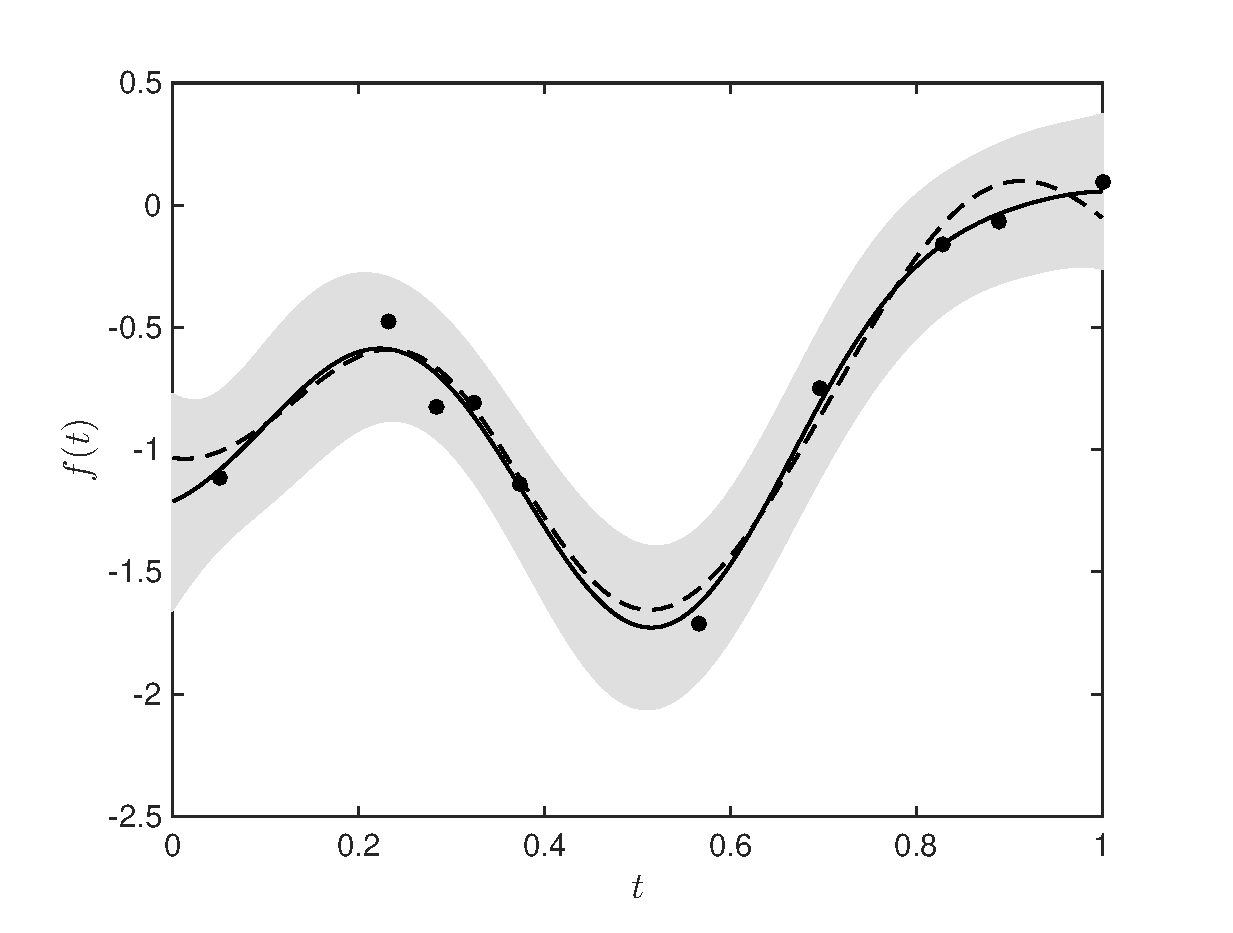
\includegraphics[width=0.9\columnwidth]{toyGPoutput}
% where an .eps filename suffix will be assumed under latex,
% and a .pdf suffix will be assumed for pdflatex; or what has been declared
% via \DeclareGraphicsExtensions.
\caption{Example of Gaussian process regression.  The dashed line represents the unknown function $f(t)$. The dots are
  the observed data $\{t_k, y_k\}_{k=1}^n$. The solid line is the posterior mean $\mu_{f(t^*) \mid \mathbf{y}}$, and the
  shaded region represents two standard deviations away from the predictive mean.}
\label{reg_ex}
\end{figure}

An additional element that is usually considered in GP regression is the estimation of the parameters of the covariance
function $k(t,t')$, also known as hyperparameters. However, the GP regression formulation allows for the following simple expression for the likelihood of measurement given the parameters:
%
\begin{equation}
  p(\mathbf{y} \mid \theta,\sigma^2)
  = \mathcal{N}(\mathbf{y} \mid \mathbf{0}, \mathbf{K}(\mathbf{t}, \mathbf{t};\theta) + \sigma^2 \mathbf{I}).
\end{equation}
%
Given the likelihood there are different ways in which the hyperparameters can be estimated, including maximization of the log-marginal likelihood \cite{Rasmussen+Williams:2006}, maximum a posteriori \cite{Murphy:2012:MLP}, and Markov chain Monte Carlo \cite{FilipponeML13}. 

\subsection{GP Regression Solution to Basic LFM Inference}\label{sec:gp:regression:lfm}
%
%\simo{Mauricio: check the notation: DONE}

Let us now consider the inclusion of a differential equation model to the Gaussian process regression. which leads to a simple latent force model. A canonical example of a linear latent force model (LFM) \cite{Alvarez+Luengo+Lawrence:2009,Alvarez+Luengo+Lawrence:2013} is the following:
%
\begin{eqnarray}
  &u(t) \sim \mathcal{GP}(0,k(t - t')), \label{eq:lgp1} \\
  &a_n \, \frac{df^{n}(t)}{dt^{n}} + \cdots
  + a_1 \, \frac{df(t)}{dt} + a_0 = u(t), \label{eq:difeq1} \\
  &y_k = f(t_k) + \epsilon_k, \label{eq:meas1}
\end{eqnarray}
%
which contains three parts: a Gaussian process part \eqref{eq:lgp1}, a differential equation part \eqref{eq:difeq1}, and a measurement model \eqref{eq:meas1}. 

Equation \eqref{eq:difeq1} can written as $\mathcal{L} \, f(t)=u(t)$, where $\mathcal{L}$ is a linear
differential operator of the form $\mathcal{L}\equiv a_n \, \frac{d}{dt^{n}} + \cdots
  + a_1 \, \frac{d}{dt} + a_0$. The differential operator $\mathcal{L}$ can be related to a so called Green's function or
impulse response $h(t)$.
%\simo{What should we actually put here?}
On the stationary stage the solution to the differential equation \eqref{eq:difeq1} can be expressed as $f(t) = \int_{-\infty}^{t} h(t - s) \, u(s) \, ds$, where $h(t)$ is the impulse response of the system. When $u(s)$ is a Gaussian process with zero mean and covariance function $k(t - t')$ then we can compute the covariance function of the process $f(t)$:
%
\begin{equation}
\begin{split}
  k_{f,f}(t, t') &=
  \int_{-\infty}^{t} \int_{-\infty}^{t'}
  h(t - s) \, h(t' - s') \, k(s - s') \, ds \, ds'.
\end{split}
\label{eq:fcov}
\end{equation}
%
Thus we can replace the problem defined by \eqref{eq:difeq1} and \eqref{eq:lgp1} with an equivalent Gaussian process regression problem
%
\begin{eqnarray}
  &f(t) \sim \mathcal{GP}(0,k_{f, f}(t, t')), \label{eq:lgp2} \\
  &y_k = f(t_k) + \epsilon_k. \label{eq:meas2}
\end{eqnarray}
%
We may be interested in computing the predictive distribution for $f(t)$ at a test point $t^*$ given the training samples.
We can then use the GP regression expressions that we saw in section \ref{sec:gp:regression}, where the covariance
function is now given by $k_{f,f}(t,t')$.


We may also be interested in computing the posterior distribution for $u^*$ at a test time point $t^*$ given noisy
measurements $y_1, \ldots, y_n$ at input times $t_1, \ldots, t_n$. To that end, we compute the cross-covariance function
between the input process $u(t)$, and the output process $f(t)$, using
\begin{align}
k_{f,u}(t,t') & = \int_{-\infty}^t h(t-s)\, k(s - t')\, ds.
\label{eq:fucov}
\end{align}
We assume then that $\mathbf{y}$ and $u^*$ are jointly Gaussian distributed, and their distribution follows
\begin{align*}
\begin{pmatrix}
\mathbf{y}\\
u^*
\end{pmatrix}\sim
\mathcal{N}
\left(
\begin{pmatrix}
\mathbf{0}\\
0
\end{pmatrix},
\begin{pmatrix}
\mathbf{K}_{f,f}(\mathbf{t}, \mathbf{t}) + \sigma^2\mathbf{I} & \mathbf{k}_{f,u}(\mathbf{t}, t^*)\\
\mathbf{k}_{f,u}^{\top}(\mathbf{t}, t^*) & k(t^*, t^*),
\end{pmatrix}
\right),
\end{align*}
where $\mathbf{K}_{f,f}(\mathbf{t}, \mathbf{t})\in\mathbb{R}^{n\times n}$ is a matrix with entries given by
$\{k_{f,f}(t_i, t_j)\}_{i=1, j=1}^{n,n}$, and $\mathbf{k}_{f,u}(\mathbf{t}, t^*) \in\mathbb{R}^{n}$ is a vector with entries
given by $\{k_{f,u}(t_i, t^*)\}_{i=1}^{n}$. Notice that due to the assumed independence between $u(t)$ and $\epsilon_k$,
the covariance between the process $y(t)$ and $u(t)$ is the same than the covariance between the process $f(t)$, and
$u(t)$.

Posterior distribution for $u^*$ given $\mathbf{y}$ follows a Gaussian distribution with mean $\mu_{u^* \mid \mathbf{y}}$, and
variance $\sigma^2_{u^* \mid \mathbf{y}}$,
\begin{align*}
\mu_{u^* \mid \mathbf{y}} & = \mathbf{k}_{f,u}^{\top}(t^*, \mathbf{t})\left[\mathbf{K}_{f,f}(\mathbf{t}, \mathbf{t})
+ \sigma^2\mathbf{I}\right]^{-1}\mathbf{y}\\
\sigma^2_{u^* \mid \mathbf{y}} & =  k(t^*, t^*) - \mathbf{k}_{f,u}^{\top}(\mathbf{t}, t^*)\left[\mathbf{K}_{f,f}(\mathbf{t}, \mathbf{t})
+ \sigma^2\mathbf{I}\right]^{-1}\mathbf{k}_{f,u}(\mathbf{t}, t^*).
\end{align*}

This approach introduced by
\cite{Alvarez+Luengo+Lawrence:2009,Alvarez+Luengo+Lawrence:2013} conveniently
reduces the original LFM into an Gaussian process regression problem
with a modified covariance function. However, the approach requires
that we need to solve the impulse response $h$ and then compute the
covariance functions via \eqref{eq:fcov}, and \eqref{eq:fucov}.  If we can obtain closed form
expressions for them, then the inference procedure becomes very
easy. Otherwise numerical computations are needed.

\subsection{State-Space ODE LFMs} \label{sec:ss_de_lfms}
%
A convenient way to compute the impulse responses required for the GP inference on LFMs is to rewrite the differential equation in state-space form, which allows us to express the impulse response in terms of matrix exponential function. We can rewrite the basic LFM differential equation \eqref{eq:difeq1} in state-space form \cite{Hartikainen+Sarkka:2011,Hartikainen+Seppanen+Sarkka:2012} by defining a state vector $\mathbf{f} = (f, df/dt,\ldots,d^{n-1}f/dt^{n-1})$ and writing
%
\begin{equation}
\begin{split}
  \frac{d\mathbf{f}(t)}{dt}
  &= \underbrace{\begin{pmatrix}
       0             & 1      &        &       \\
                     & \ddots & \ddots &       \\
                     &         &  0    &     1 \\
   -a_0 & -a_1 & \hdots &  -a_{n-1}
  \end{pmatrix}}_{\mathbf{A}_f} \, \mathbf{f}(t)
  + \underbrace{\begin{pmatrix}
      0 \\
      \vdots \\
      0 \\
      \frac{1}{a_n}
  \end{pmatrix}}_{\mathbf{B}_f} \,
   u(t) \\
   f(t) &= \underbrace{\begin{pmatrix}
     1 & 0 & \cdots & 0
   \end{pmatrix}}_{\mathbf{C}_f} \, \mathbf{f}(t)
\end{split}
\label{eq:ss1}
\end{equation}
%
This gives the following state-space representation for $f(t)$:
%
\begin{equation}
\begin{split}
  \frac{d\mathbf{f}(t)}{dt}
  &= \mathbf{A}_f \, \mathbf{f}(t) + \mathbf{B}_f \, u(t) \\
  f(t) &= \mathbf{C}_f \, \mathbf{f}(t).
\end{split}
\label{eq:ssgen}
\end{equation}
%
Because this system is of the first order, the impulse response---which is now a matrix valued function---can be written down explicitly in terms of the matrix exponential function $\mathbf{H}(t) = \exp(t \, \mathbf{A}_f)$ and hence the joint covariance function of $\mathbf{f}$ is
%
\begin{equation}
\begin{split}
  &\mathbf{K}_\mathbf{f}(t - t')
  \\ &
  =
  \int_{-\infty}^{t} \int_{-\infty}^{t'}
  \mathbf{H}(t - s) \, \mathbf{B}_f \, k(s - s') \,
  \mathbf{B}_f^{\top} \, \mathbf{H}^{\top}(t' - s') \, ds \, ds',
\end{split}
\label{eq:vfcov}
\end{equation}
%
and we can pick up the covariance function of $f(t)$ from the matrix via
%
\begin{equation}
\begin{split}
  k_f(t,t') &=
  \mathbf{C}_f \, \mathbf{K}_\mathbf{f}(t - t') \, \mathbf{C}_f^{\top}
\end{split}
\label{eq:fcov2}
\end{equation}
%
The required cross-variance $k_{f,u}$ can be compute by form noting that
%
\begin{equation}
\begin{split}
  &\mathbf{K}_{\mathbf{f},u}(t - t')
%  \\ &
  =
  \int_{-\infty}^{t} 
  \mathbf{H}(t - s) \, \mathbf{B}_f \, k(s - t') \, ds,
\end{split}
\label{eq:vfucov}
\end{equation}
%
which further gives
%
\begin{equation}
\begin{split}
  k_{f,u}(t,t') &=
  \mathbf{C}_f \, \mathbf{K}_{\mathbf{f},u}(t - t').
\end{split}
\label{eq:fucov2}
\end{equation}

These representations have the advantage that it is easy to numerically approximate the matrix exponential and hence the analytical computation of the impulse response becomes unnecessary. However, we still need to compute the integrals in \eqref{eq:vfcov} and \eqref{eq:vfucov} somehow. If closed form solution is not available (which surprising often is), then the computations need to be done via numerical integration.

Later in this article we consider state-space methods which also convert the variance function $k(t,t')$ into a (stochastic) differential equation form. In that kind of formulation we are able to avoid the numerical integration altogether and replace it with matrix exponential computations and solutions to Lyapunov equations, which are numerically easier tasks.


%\simo{Simo: Explain how to get $k_{f,u}$}

\subsection{Partial Differential Equation Based LFMs}
%
Similar to the case of ordinary differential equations, we can associate a Green's function to a linear partial differential operator \cite{Myintu:LPDEBook:2006, Polyanin:Handbook02}.\footnote{The presentation here refers to boundary value problems.} Let $H(\mathbf{x}, \mathbf{x}')$ be the Green's function for a particular linear partial differential operator, where $\mathbf{x}$ is a general input vector that could include different types of input variables, as we mentioned before. For example, the vector $\mathbf{x}$ could refer to coordinates $x$ and $y$ for the Poisson equation in two spatial dimensions, or to coordinate $x$ and time $t$ for the Heat equation in one spatial dimension.

For example, the Poisson equation is given as
\begin{align*}
  \nabla^2 f(\mathbf{x}) = u(\mathbf{x}).
\end{align*}
%
The solution for $f(\mathbf{x},t)$ has the form
\begin{align*}
f(\mathbf{x}) & = \int_{\mathcal{X}} H(\mathbf{x}, \mathbf{z})\,
                u(\mathbf{z})\,d\mathbf{z} + g(\mathbf{x}),
\end{align*}
%
where $\mathcal{X}$ is the input domain of integration, and $g(\mathbf{x})$ is the solution due to the boundary conditions. For simplicity in the presentation, we assume that the boundary conditions are zero, but the boundary conditions could also be incorporated. In this case the Green's function $H(\mathbf{x}, \mathbf{z})$, with suitable boundary conditions, can be written in closed form. The expression for this Green's function can be found in \cite{Polyanin:Handbook02}. 
%\simo{Mauricio: Find a citation for this closed form expression DONE}

For the GP regression view of latent force models, we put a GP prior over $u(\mathbf{x})$,
\begin{align*}
u(\mathbf{x})\sim\mathcal{GP}(0, k(\mathbf{x} - \mathbf{x}')).
\end{align*}
Covariance for $f(\mathbf{x})$ then follows a similar expression to \eqref{eq:fcov},
\begin{equation}
\begin{split}
  k_{f,f}(\mathbf{x}, \mathbf{x}') &=
  \int_{\mathcal{X}}   \int_{\mathcal{X}}
  H(\mathbf{x}, \mathbf{z}) \, H(\mathbf{x}', \mathbf{z}') \, k(\mathbf{z} - \mathbf{z}') \, d\mathbf{z} \, d\mathbf{z}'.
\end{split}
\notag
%\label{eq:fcov:pde}
\end{equation}
Cross-covariance between the output process $f(\mathbf{x})$, and the input process $u(\mathbf{x})$ can also be computed
using a similar expression to \eqref{eq:fucov}
\begin{align}
k_{f,u}(\mathbf{x},\mathbf{x}') & = \int_{\mathcal{X}} H(\mathbf{x}, \mathbf{z})\, k(\mathbf{z} - \mathbf{x}')\, d\mathbf{z}.
\notag
%\label{eq:fucov}
\end{align}
Based on a set of noisy training samples, $\mathcal{D}=\{\mathbf{x}_k, y_k\}_{k=1}^n$, we can
use the GP regression equations in Sections \ref{sec:gp:regression} and \ref{sec:gp:regression:lfm}, to make predictions
for a test input $\mathbf{x}^*$, both for the output process $f(\mathbf{x})$, and the input process $u(\mathbf{x})$.

As an example of spatio-temporal PDE, the heat equation is given as
\begin{align*}
  \frac{\partial f(\mathbf{x},t)}{\partial t} &= D \, \nabla^2 f(\mathbf{x},t) - \beta \, f(\mathbf{x},t) + u(\mathbf{x},t).
\end{align*}
%
Let us now assume that we have an initial value problem (i.e., a Cauchy problem) with zero initial condition $f(\mathbf{x},t_0) = 0$ at a fixed $t_0$ together with certain boundary conditions on the boundary of a domain $\mathcal{X}$. 

The solution for $f(\mathbf{x},t)$ can be written as
\begin{align*}
f(\mathbf{x},t) & = \int_{t_0}^t \int_{\mathcal{X}} H(\mathbf{x}, t;  \mathbf{z}, s)\,
                u(\mathbf{z},s)\,d\mathbf{z}\,ds
\end{align*}
%
and again the Green's function $H$ it can be written in closed form. See \cite{Polyanin:Handbook02} for the particular expression. 

In this case the Green's function is also the kernel of so called operator exponential (exponential semigroup) of the operator:
%
\begin{equation}
  \mathcal{H}(t, s) = \exp\left( (t-s) \, (D \, \nabla^2 - \beta) \right).
\end{equation}
%
The covariance functions of the process can now be expressed in terms of the Green's function
%
\begin{equation}
\begin{split}
  &k_{f,f}(\mathbf{x}, t; \mathbf{x}', t') \\
  &=
  \int_{t_0}^{t'} \int_{\mathcal{X}} \int_{t_0}^{t}  \int_{\mathcal{X}} 
  H(\mathbf{x}, t; \mathbf{z}, s) \,
  H(\mathbf{x}', t'; \mathbf{z}', s') \\ 
   &\qquad \qquad \qquad \times
  k(\mathbf{z}, s; \mathbf{z}', s') \, d\mathbf{z} \, ds \, d\mathbf{z}' \, ds' \\
  &k_{f,u}(\mathbf{x}, t; \mathbf{x}', t') \\
  &=
  \int_{t_0}^{t}  \int_{\mathcal{X}} 
  H(\mathbf{x}, t; \mathbf{z}, s) \,
  k(\mathbf{z}, s; \mathbf{x}', t') \, d\mathbf{z} \, ds 
\end{split}
\notag
\end{equation}
%
The above approach conveniently generalizes to Gaussian process driven partial (or pseudo-differential) equations of the form (cf. \cite{Sarkka:2011})
\begin{align*}
  \mathcal{D} f(\mathbf{x},t) = u(\mathbf{x},t),
\end{align*}
%
where $\mathcal{D}$ is a (pseudo) differential operator.

Once we have derived the covariance functions, we can use the Gaussian process regression equations as in Sections \ref{sec:gp:regression} and \ref{sec:gp:regression:lfm} for learning and prediction of functions $f$ and $u$.

\subsection{State-Space PDE LFMs}

We can also extend the ideas presented in Section~\ref{sec:ss_de_lfms} to the spatial-temporal case.  Assume that that our PDE LFM has the form
%
\begin{equation}
\begin{split}
  \frac{\partial \mathbf{f}(\mathbf{x},t)}{\partial t}
  &= \mathbf{\mathcal{A}}_f \, \mathbf{f}(\mathbf{x},t) + \mathbf{B}_f \, u(\mathbf{x},t), \\
\end{split}
\end{equation}
%
where $\mathbf{\mathcal{A}}_f$ is a matrix of linear operators. Let the covariance function of $u$ be $k(\mathbf{x},\mathbf{x}';t - t')$. Then, if we define the operator exponential (or the impulse response) as $\mathbf{\mathcal{H}}(t) = \exp(t \, \mathbf{\mathcal{A}_f})$, the covariance function of $f$ can be expressed as
%
\begin{equation}
\begin{split}
  k_f(\mathbf{x},\mathbf{x}';t-t') &=
  \mathbf{C}_f \, \mathbf{K}_\mathbf{f}(\mathbf{x},\mathbf{x}';t-t') \, \mathbf{C}_f^{\top}
\end{split}
\end{equation}
%
with
%
\begin{equation}
\begin{split}
  &\mathbf{K}_\mathbf{f}(\mathbf{x},\mathbf{x}';t-t')
  \\ &
  =
  \int_{-\infty}^{t} \int_{-\infty}^{t'}
  \mathbf{\mathcal{H}}(t - s) \, \mathbf{B}_f \, k(\mathbf{x},\mathbf{x}';s - s') \,
  \mathbf{B}_f^{\top} \, \mathbf{\mathcal{H}}^{\top}(t' - s') \, ds \, ds',
\end{split}
\label{eq:vfcov_pde}
\end{equation}
%
where the operator multiplication from right is interpreted as acting onto the variable $\mathbf{x}'$. The
\mauricio{cross-variance cross-covariance?} between $f$ and $u$ has the representation
%
\begin{equation}
\begin{split}
  k_{f,u}(\mathbf{x},\mathbf{x}';t-t') &=
  \mathbf{C}_f \, 
  \int_{-\infty}^{t}
  \mathbf{\mathcal{H}}(t - s) \, \mathbf{B}_f \, k(\mathbf{x},\mathbf{x}';s - t') \, ds.
\end{split}
\end{equation}

\subsection{Hyperparameter Learning in LFMs}

Expressions for the covariance functions $k_{f}(t,t')$, $k_{f}(\mathbf{x}, \mathbf{x}', t-t')$, and $k_{f}(\mathbf{x}, \mathbf{x}')$ also involve the parameters of the differential equations, and the parameters of the covariance function of the latent process $u(\cdot)$. Once we have formed the GP model with the modified covariance function, those hyperparameters can be estimated using any of the methods mentioned in the section on GP regression. In the context of latent force models, there have been more recent
attempts to estimate these hyperparameters using Markov Chain Monte Carlo, by including priors for the parameters of the differential equations and the covariance function of the latent process \cite{Titsias:control:vars:2009, Titsias:BMC:2012}.


\section{Latent Force Models as Stochastic State-Space Models}

In this section, we discuss state-space methods for Gaussian process regression and especially show how they can be used with latent force models. 

\subsection{Temporal GPs in state-space form} \label{sec:tempgp}
As shown in \cite{Hartikainen+Sarkka:2010,Sarkka+Solin+Hartikainen:2013,Sarkka+Piche:2014} many covariance function based models of the form
%
\begin{equation}
  u(t) \sim \mathcal{GP}(0,k(t - t'))
\end{equation}
%
can be equivalently or approximately expressed in state-space form by defining a state vector such as $\mathbf{u} = (u,
du/dt,\ldots,d^{p-1}u/dt^{p-1})$---note that depending on parameterization the state vector might not contain exactly
the derivatives, but \mauricio{\textbf{something related} I'm not sure I understand this}---leading to a state-space model
%
\begin{equation}
\begin{split}
  \frac{d\mathbf{u}(t)}{dt}
  &= \mathbf{A}_u \, \mathbf{u}(t) + \mathbf{B}_u \, w(t) \\
  u(t) &= \mathbf{C}_u \, \mathbf{u}(t),
\end{split}
\label{eq:ssu}
\end{equation}
%
where $w(t)$ is a white-noise process. The advantage of \mauricio{\textbf{this kind} maybe too informal?} of model formulation is that it allows for solving the GP regression problem using Kalman filters and smoothers \cite{Sarkka:2013} in $O(n)$ time when the traditional GP takes $O(n^3)$ time (here $n$ denotes the number of measurements).

The key (classical) result is that such a white-noise-driven state-space representation exists if and only if the spectral density (the Fourier transform of $k(\tau)$) is a proper rational function:
%
\begin{equation}
\begin{split}
  S(\omega) &= \frac{d_0 + d_1 \, \omega^2 + \cdots + d_r \, \omega^{2r}}{c_0 + c_1 \, \omega^2 + \cdots + c_s \, \omega^{2s}}.
\end{split}
\end{equation}
%
By using the spectral factorization and classical state-space realizations \cite{Sarkka+Solin+Hartikainen:2013} it is then possible to construct the matrices $\mathbf{A}_u$, $\mathbf{B}_u$, and $\mathbf{C}_u$ such that $u(t)$ has the desired covariance function. 

For example, the Mat\'ern covariance functions  $k(\tau) = \left( \sigma^2 \, 2^{1-\nu} / \Gamma(\nu)\right) \left(\sqrt{2\nu}\,\tau / \ell \right)^\nu K_\nu\left(\sqrt{2\nu}\,\tau / \ell \right)$ with certain parameter values ($\nu=1/2,3/2,\ldots$) have exact state-space representations. In particular, with $\nu=3/2$ we get
 %
\begin{equation}
\begin{split}
\frac{d\mathbf{u}(t)}{dt} &= \underbrace{\begin{pmatrix} 0 & 1 \\ -\lambda^2 & -2\lambda \end{pmatrix}}_{\mathbf{A}_u}
 \, \mathbf{u}(t)
+ \underbrace{\begin{pmatrix} 0 \\ 1 \end{pmatrix}}_{\mathbf{B}_u} \, w(t), \\
   u(t) &= \underbrace{\begin{pmatrix} 1 & 0 \end{pmatrix}}_{\mathbf{C}_u} \, \mathbf{u}(t),
\end{split}
\end{equation}
%
where $\lambda=\sqrt{2\nu}/\ell$. 

Although the commonly used squared exponential covariance function does not have an exact state-space representation, it
can be easily approximated \mauricio{\textbf{with such} ??} using a simple Taylor series expansions or Pad\'e approximants in Fourier domain \cite{Sarkka+Piche:2014,Karvonen+Sarkka:2016}. State-space representations of periodic covariance functions have been considered in \cite{Solin+Sarkka:2014a}, and rational quadratic and general scale mixtures of Gaussians in \cite{Solin+Sarkka:2014b}. A review of different representations and approximations can be found in \cite{Solin:2016}.

To some extent it is also possible to convert non-stationary covariance function into state space form. However, in that case the Fourier domain approach above is not applicable. For example, Wiener processes and $n$-times integrated Wiener processes are non-stationary Gaussian processes, but they still have easy state-space representation (see, e.g., \cite{Solin:2016}). There also exists some general procedures (e.g., \cite{Anderson:1969,Van-Trees:1971}) for converting non-stationary covariance functions into state-space form.

\subsection{Spatio-temporal GPs in state-space form}

It is also possible to extend the above concepts to spatio-temporal covariance functions of the form $k(\mathbf{x} - \mathbf{x}', t-t')$, which in turn gives covariance functions $k(\mathbf{x} - \mathbf{x}')$ as a special case, because we can always reinterpret one of the components of $\mathbf{x}$ as time. The methods to form these infinite-dimensional state-space representations have been considered in \cite{Sarkka+Hartikainen:2012,Sarkka+Solin+Hartikainen:2013}. 

The conversion of a spatio-temporal covariance function into state-space form leads to a system of the form
%
\begin{equation}
\begin{split}
  \frac{\partial\mathbf{u}(\mathbf{x},t)}{\partial t} &= \mathbf{\mathcal{A}}_u \, \mathbf{u}(\mathbf{x},t)
  + \mathbf{B}_u \, w(\mathbf{x},t) \\
   u(\mathbf{x},t) &= \mathbf{C}_u \, \mathbf{u}(\mathbf{x},t),
\end{split}
\label{eq:ssu2}
\end{equation}
%
where $\mathbf{\mathcal{A}}_u$ is a matrix of linear operators (typically pseudo-differential operators) acting on the $\mathbf{x}$-variable and $w(\mathbf{x},t)$ is a time-white spatio-temporal Gaussian process.

The representation can be obtained, for example, by an extension of the spectral factorization based method to the temporal case. We can first form the joint space-time spectral density $S(\boldsymbol{\omega}_{\mathbf{x}},\omega_t)$ and approximate it as
%
\begin{equation}
\begin{split}
  S(\boldsymbol{\omega}_{\mathbf{x}},\omega_t)
  \approx   \frac{d_0(\boldsymbol{\omega}_{\mathbf{x}})
  + d_1(\boldsymbol{\omega}_{\mathbf{x}}) \, \omega_t^2
  + \cdots + d_r(\boldsymbol{\omega}_{\mathbf{x}}) \, \omega_t^{2r}}
  {c_0(\boldsymbol{\omega}_{\mathbf{x}}) + c_1(\boldsymbol{\omega}_{\mathbf{x}}) \, \omega_t^2
  + \cdots + c_s(\boldsymbol{\omega}_{\mathbf{x}}) \, \omega_t^{2s}}.
\end{split}
\end{equation}
%
The spectral factorization in variable $\omega_t$ then leads to a temporal state space model, where the matrices depend on the spatial frequency $\boldsymbol{\omega}_{\mathbf{x}}$. A spatial inverse Fourier transform then transforms the terms into linear operators leading to a model of the form \eqref{eq:ssu2}. More details can be found in \cite{Sarkka+Solin+Hartikainen:2013}.

For example, the spatio-temporal Mat\'ern covariance function with a suitable parametrization leads to the following representation \cite{Sarkka+Solin+Hartikainen:2013}:
%
\begin{equation}
\begin{split}
  \frac{\partial \mathbf{u}(\mathbf{x},t)}{\partial t} &= 
       \underbrace{\begin{pmatrix} 
        0 & 1 \\ 
        \nabla^2-\lambda^2
        & -2 \sqrt{\lambda^2-\nabla^2} 
      \end{pmatrix}}_{\mathbf{\mathcal{A}}_u} \mathbf{u}(\mathbf{x},t)
      + \underbrace{\begin{pmatrix} 0 \\ 1 \end{pmatrix}}_{\mathbf{B}_u} w(\mathbf{x},t), \\
      u(\mathbf{x},t) &= \underbrace{\begin{pmatrix} 1 & 0 \end{pmatrix}}_{\mathbf{C}_u} \, \mathbf{u}(\mathbf{x},t),
\end{split}
\label{2dmatern_ss}
\end{equation}
%
where $\nabla^2 = \partial^2 / \partial x_1^2 + \cdots + \partial^2 / \partial x_p^2$ and $\sqrt{\cdot}$ in the matrix $\mathbf{\mathcal{A}}_u$ denotes an operator square root.

State-space realizations of spatio-temporal oscillating fields have been discussed in \cite{Solin+Sarkka:2013}. The implementation of divergence-free covariance functions for magnetic field modeling have been recently presented in \cite{Solin:2017}. It is worth noting that fixing the GP to be realized as its causal version via the spectral factorization can also cause problems when the GP is combined with a suitable non-causal PDE. This is discussed in Section~\ref{sec:poisson-problem}.

As in the case of temporal processes discussed in Section~\ref{sec:tempgp}, it is possible to convert some classes of non-stationary covariance functions in state-space form. In that case the Fourier domain approach is not applicable, but similar methods as in the temporal case can also be used for spatio-temporal models.


\subsection{ODE LFMs in joint state-space form}
%
We can now combine the  state-space ODE \eqref{eq:ssgen} with the state-space representation of LFMs in the previous section to obtain an augmented state-space representation of the LFM \cite{Hartikainen+Sarkka:2011,Hartikainen+Seppanen+Sarkka:2012}. Thus we obtain a combined model
%
\begin{equation}
\begin{split}
  \frac{d\mathbf{f}(t)}{dt}
  &= \mathbf{A}_f \, \mathbf{f}(t)
  + \mathbf{B}_f \, \mathbf{C}_u \, \mathbf{u}(t) \\
  \frac{d\mathbf{u}(t)}{dt}
  &= \mathbf{A}_u \, \mathbf{u}(t) + \mathbf{B}_u \, w(t) \\
  f(t) &= \mathbf{C}_f \, \mathbf{f}(t).
\end{split}
\label{eq:comb}
\end{equation}
%
If we now define
%
\begin{equation}
\begin{split}
  \mathbf{g} &= \begin{pmatrix}
	\mathbf{f} \\ \mathbf{u}
  \end{pmatrix}, \quad
  \mathbf{A}
  = \begin{pmatrix}
	\mathbf{A}_f & \mathbf{\mathbf{B}_f \, \mathbf{C}_u} \\
	0 & \mathbf{A}_u
  \end{pmatrix} \\
  \mathbf{B}
  &= \begin{pmatrix}
	0 & \mathbf{B}_u
  \end{pmatrix}, \quad
  \mathbf{C}
  = \begin{pmatrix}
	\mathbf{C}_f & 0
  \end{pmatrix}
\end{split}
\label{eq:ssaugmats}
\end{equation}
%
then the model can be written as a white-noise driven state-space model
%
\begin{equation}
\begin{split}
  \frac{d\mathbf{g}(t)}{dt}
  &= \mathbf{A} \, \mathbf{g}(t)
  + \mathbf{B} \, w(t) \\
  f(t) &= \mathbf{C} \, \mathbf{g}(t).
\end{split}
\label{eq:ssaug}
\end{equation}
%
The measurements can be included into the model by replacing the second equation above by
%
\begin{equation}
\begin{split}
  y_k &= \mathbf{C} \, \mathbf{g}(t_k) + \epsilon_k.
\end{split}
\label{eq:ssaugkf}
\end{equation}
%
The advantage of this formulation is that we can infer both the process and the latent Gaussian process via Kalman
filtering and smoothing in linear time (see \cite{Hartikainen+Sarkka:2010,Sarkka+Solin+Hartikainen:2013}). The link to
Kalman filtering and smoothing follows from the result that as the model above is linear, we can form an exact
discretization of the model as
%
\begin{equation}
\begin{split}
  \mathbf{g}_k
  &= \mathbf{U}(\Delta t_k) \, \mathbf{g}_{k-1}
  + \mathbf{q}_k \\
  y_k &= \mathbf{C} \, \mathbf{g}_k + \epsilon_k.
\end{split}
\label{eq:dssaug}
\end{equation}
%
where $\mathbf{g}_k \triangleq \mathbf{g}(t_k)$, $\mathbf{q}_k \sim \mathcal{N}(0,\mathbf{Q}(\Delta t_k)$, $\Delta_t = t_k - t_{k-1}$, and
%
\begin{equation}
\begin{split}
  \mathbf{U}(\Delta t_k)  &= \exp(\Delta t_k \, \mathbf{A}), \\
  \mathbf{Q}(\Delta t_k) &= \int_0^{\Delta t_k} \exp((\Delta t_k - \tau) \, \mathbf{A}) \,
  \mathbf{B} \, q_c  \, \mathbf{B}^{\top} \\
  &\qquad \quad \times \exp((\Delta t_k - \tau) \, \mathbf{A})^{\top} \, d\tau,
\end{split}
\label{eq:dssaug}
\end{equation}
%
where $q_c$ is the spectral density of the white noise $w(t)$. For numerical computation of the matrix exponential and the above integral there exists a wide range of numerical methods (see, e.g., \cite{Grewal+Andrews:2001,Sarkka:2006}) with ready-available implementations.

The link to Kalman filtering results from the fact that the model \mauricio{\eqref{eq:dssaug} until this point, the
  equation has not been introduced} is a standard discrete-time linear Gaussian model and the Kalman filter and (Rauch--Tung--Striebel, RTS) smoother provide the equations for exact Bayesian inference on it (see, e.g., \cite{Sarkka:2013}). 

Another benefit of the representation \eqref{eq:comb} is that we can compute the covariance functions corresponding to the ODE LFM without resorting to numerical integration as in \eqref{eq:fcov} and \eqref{eq:fucov}, or \eqref{eq:vfcov} and \eqref{eq:vfucov}. The joint stationary covariance function of $\mathbf{g}(t) = (\mathbf{f}(t),\mathbf{u}(t))$ can be expressed as
%
\begin{equation}
\begin{split}
  \mathbf{K}_{\mathbf{g}}(t,t') = \begin{cases}
    \mathbf{P}_\infty \, \exp(( t - t') \, \mathbf{A})^{\top}, &
    \text{ if } t \ge t' \\
    \exp((t' - t) \, \mathbf{A}) \, \mathbf{P}_\infty, &
    \text{ if } t < t',
  \end{cases}
\end{split}
\label{eq:Kg1}
\end{equation}
%
where $\mathbf{P}_\infty$ is the solution to the Lyapunov equation
%
\begin{equation}
\begin{split}
  \mathbf{A} \, \mathbf{P}_\infty + \mathbf{P}_\infty \, \mathbf{A}^{\top}
  + \mathbf{B} \, q_c \, \mathbf{B}^{\top} = 0.
\end{split}
\label{eq:Kg2}
\end{equation}
%
We can then pick up the covariance function of $f$ and the cross-covariance of $f$ and $u$ as
%
\begin{equation}
\begin{split}
  k_{f,f}(t,t') = \mathbf{C} \, \mathbf{K}_{\mathbf{g}}(t,t') \, \mathbf{C}^{\top}, \\
  k_{f,u}(t,t') = \mathbf{C} \, \mathbf{K}_{\mathbf{g}}(t,t') \, \mathbf{D}^{\top}, \\
\end{split}
\label{eq:Kg3}
\end{equation}
%
where we have defined $\mathbf{D} = \begin{pmatrix} 0 & \mathbf{C}_u \end{pmatrix}$.


\subsection{PDE LFMs in joint state-space form}
%
Partial differential equation models driven by Gaussian processes can also be often represented in a similar state-space form as the temporal models considered in the previous section. Consider for example the heat equation
%
\begin{equation}
\begin{split}
  \frac{\partial f(\mathbf{x},t)}{\partial t} &=
  D \, \nabla^2 \, f(\mathbf{x},t) - \beta \, f(\mathbf{x},t) + u(\mathbf{x},t) \\
\end{split}
\end{equation}
%
Let us now assume that we are have a state-space representation of the unknown function $u(\mathbf{x},t)$ in form \eqref{eq:ssu2}. This thus leads to the system
%
\begin{equation}
\begin{split}
  \frac{\partial f(\mathbf{x},t)}{\partial t} &=
  \underbrace{\left( D \, \nabla^2 - \beta \right)}_{\mathbf{\mathcal{A}}_f} \, f(\mathbf{x},t) + \mathbf{C}_u \, \mathbf{u}(\mathbf{x},t) \\
  \frac{\partial\mathbf{u}(\mathbf{x},t)}{\partial t} &= \mathbf{\mathcal{A}}_u \, \mathbf{u}(\mathbf{x},t)
  + \mathbf{B}_u \, w(\mathbf{x},t) \\
\end{split}
\end{equation}
%
where the analogy to the model \eqref{eq:comb} is apparent. For higher order derivatives on the left hand side we should define a vector of derivatives $\begin{pmatrix} f, \partial f/\partial t, \ldots \end{pmatrix}$, but for the present first order case this is unnecessary.

In order to obtain a single augmented model, analogously to the previous section we can define (with $\mathbf{B}_f = 1$ in this particular case)
%
\begin{equation}
\begin{split}
  \mathbf{g} &= \begin{pmatrix}
	\mathbf{f} \\ \mathbf{u}
  \end{pmatrix}, \quad
  \mathbf{\mathcal{A}}
  = \begin{pmatrix}
	\mathbf{\mathcal{A}}_f & \mathbf{B}_f \, \mathbf{C}_u \\
	0 & \mathbf{\mathcal{A}}_u
  \end{pmatrix} \\
  \mathbf{B}
  &= \begin{pmatrix}
	0 & \mathbf{B}_u
  \end{pmatrix}, \quad
  \mathbf{C}
  = \begin{pmatrix}
	1 & 0
  \end{pmatrix}
\end{split}
\end{equation}
%
which leads to a model of the form
%
\begin{equation}
\begin{split}
  \frac{\partial \mathbf{g}(\mathbf{x},t)}{\partial t}
  &= \mathbf{\mathcal{A}} \, \mathbf{g}(\mathbf{x},t)
  + \mathbf{B} \, w(\mathbf{x},t) \\
  y_k &= \mathbf{C} \, \mathbf{g}(t_k) + \epsilon_k.
\end{split}
\label{eq:ssaug2}
\end{equation}
%
The discretization now proceeds analogously to the previous section, except that the matrix exponential is replaced with an operator exponential (exponential semigroup) and its time-integral:
%
\begin{equation}
\begin{split}
  \mathbf{\mathcal{U}}(\Delta t_k)  &= \exp(\Delta t_k \, \mathbf{\mathcal{A}}), \\
  \mathbf{Q}(\mathbf{x},\mathbf{x}';\Delta t_k) &= \int_0^{\Delta t_k} \exp((\Delta t_k - \tau) \, 
  \mathbf{\mathcal{A}}) \,
  \mathbf{B} \, q_c(\mathbf{x},\mathbf{x}')  \, \mathbf{B}^{\top} \\
  &\qquad \quad \times \exp((\Delta t_k - \tau) \, \mathbf{\mathcal{A}})^{\top} \, d\tau.
\end{split}
\label{eq:dssaug}
\end{equation}
%
Furthermore, both the spectral density $q_c(\mathbf{x},\mathbf{x}')$ and the covariance $\mathbf{Q}(\mathbf{x},\mathbf{x}';\Delta t_k)$ become kernels in $\mathbf{x},\mathbf{x}'$. Note that above, we need to interpret the operator application from the right as operating onto the variable $\mathbf{x}'$ (cf. \cite{Sarkka+Hartikainen:2012}).

The inference in the above model can be done with infinite-dimensional Kalman filters and RTS smoothers (see, \cite{Sarkka+Hartikainen:2012}). However, in practice we often use some kind of basis function expansion methods to project the equations onto a finite-dimensional sub-space which reduces the filters and smoothers to their finite-dimensional versions.

The covariance functions for explicit GP inference could also be computed with the operator analogs of Equations \eqref{eq:Kg1}, \eqref{eq:Kg2}, and \eqref{eq:Kg3}.

\subsection{Parameter estimation in state-space LFMs}
%
In the conversion of the LFM into a state-space form, the parameters of the differential equations and covariance functions transform into parameters of the state-space model. In the resulting model we can estimate the parameters using parameter estimation methods for state-space models. See, for example, \cite{Sarkka:2013} for a review of parameter estimation methods for state-space models.

\subsection{Counter-example: the Poisson equation} \label{sec:poisson-problem}

The state-space representation has one hard limitation in the physical model: it needs to be causal in the time-direction. Although statistics of the LFM GP do not depend on the causality of the process and thus we can always replace the LFM GP with its causal version, this is not true for a physical process as we demonstrate in this section.

Sometimes we are interested in partial differential equations without time-dependence, with a prototypical example being the Poisson equation
%
\begin{equation}
\begin{split}
  \nabla^2 f(\mathbf{x}) = u(\mathbf{x})
\end{split}
\end{equation}
%
Although there is no time-variable, we can redefine one of the spatial variables as time $\mathbf{x} \triangleq (\mathbf{x},t)$ which thus leads to the equation
%
\begin{equation}
\begin{split}
  \frac{\partial^2 f(\mathbf{x},t)}{\partial t^2} + \nabla^2 f(\mathbf{x},t) = u(\mathbf{x},t)
\end{split}
\label{ipoisson}
\end{equation}
%
However, this kind of equations without builtin physical time-dependence need to more care than physically time dependent equations as will be illustrated in the following.

It would now be tempting to move the term $\nabla^2 f(\mathbf{x},t)$ to the right hand side and form a state-space form via defining the state as $\mathbf{f} = (f,\partial f/\partial t)$, which formally gives:
%
%   d2f/dt2 = -D^2 f + u
% 
%    df1/dt = f2
%    df2/dt = -D^2 f1 + u
%
\begin{equation}
\begin{split}
  \frac{\partial \mathbf{f}(\mathbf{x},t)}{\partial t} &= 
       \begin{pmatrix} 
        0 & 1 \\ 
        -\nabla^2 & 0
      \end{pmatrix} \, \mathbf{f}(\mathbf{x},t)
      + \begin{pmatrix} 0 \\ 1 \end{pmatrix} \, u(\mathbf{x},t).
\end{split}
\label{eq:noncausal-ss}
\end{equation}
%
However, this is not a valid state-space model, because it is not causal. This can be easiest seen by taking the spatial Fourier transform of \eqref{eq:noncausal-ss} which gives
%
\begin{equation}
\begin{split}
%  \frac{\partial^2 \tilde{u}(i \boldmath{\omega}_x,t)}{\partial t^2}
%  = \| \boldmath{\omega}_x \|^2 \tilde{u}(i \boldmath{\omega}_x,t) + \tilde{u}(i \boldmath{\omega}_x,t)
  \frac{\partial \tilde{\mathbf{f}}(i \boldmath{\omega}_\mathbf{x},t)}{\partial t} &= 
       \begin{pmatrix} 
        0 & 1 \\ 
        \| \boldmath{\omega}_{\mathbf{x}} \|^2 & 0
      \end{pmatrix} \, \tilde{\mathbf{f}}(i \boldmath{\omega}_\mathbf{x},t)
      + \begin{pmatrix} 0 \\ 1 \end{pmatrix} \, \tilde{u}(i \boldmath{\omega}_\mathbf{x},t).
\end{split}
\end{equation}
%
which can be seen to correspond to a unstable system, because the transition matrix has the positive eigenvalue $\| \boldmath{\omega}_{\mathbf{x}} \|$, which implies a diverging solution.

In order to form a valid state-space model, let us take time-space Fourier transform of \eqref{ipoisson} which gives
%
\begin{equation}
\begin{split}
  (i \omega_t)^2 \, F(i \boldmath{\omega}_x,i \omega_t)
  + \| i \boldmath{\omega}_x \|^2 F(i \boldmath{\omega}_x,i \omega_t)= U(i \boldmath{\omega}_x,i \omega_t)
\end{split}
\end{equation}
%
%
which implies that the spectral density of $f$ has the form
%
\begin{equation}
\begin{split}
  S_f(\boldmath{\omega}_x,\omega_t)
  &= \frac{S_u(\boldmath{\omega}_x,\omega_t)}{\left( (\omega_t)^2 \ + \| \boldmath{\omega}_x \|^2 \right)^2}
\end{split}
\end{equation}
%
which can be refactored with respect to $\omega_t$ to give the stable, statistically equivalent system
%
\begin{equation}
\begin{split}
  \frac{\partial^2 f(\mathbf{x},t)}{\partial t^2}
  + 2 \sqrt{-\nabla^2} \, \frac{\partial f(\mathbf{x},t)}{\partial t} - \nabla^2 f(\mathbf{x},t) = u(\mathbf{x},t)
\end{split}
\label{spoisson}
\end{equation}
%
which has the state-space representation
%
\begin{equation}
\begin{split}
  \frac{\partial \mathbf{f}(\mathbf{x},t)}{\partial t} &= 
       \underbrace{\begin{pmatrix} 
        0 & 1 \\ 
        \nabla^2
        & -2 \sqrt{-\nabla^2} 
      \end{pmatrix}}_{\mathbf{\mathcal{A}}_f} \mathbf{f}(\mathbf{x},t)
      + \underbrace{\begin{pmatrix} 0 \\ 1 \end{pmatrix}}_{\mathbf{B}_f} u(\mathbf{x},t), \\
      f(\mathbf{x},t) &= \underbrace{\begin{pmatrix} 1 & 0 \end{pmatrix}}_{\mathbf{C}_f} \, \mathbf{f}(\mathbf{x},t).
\end{split}
\end{equation}
%
This model is now time-stable and can be augmented with a state-space model for $u$ in order to yield a state-space representation for the full LFM model.

However, it turns out that although we can indeed estimate the process $f$ easily using the representation, the estimation of $u$ becomes non-trivial. This is because we have implicitly made a unitary transformation for the input process. Although this does not affect the covariance structure of the input, it does transform the posterior mean of it using the same transformation. In order to determine the original $u$ from the estimate of $u$ obtained from this equation, we need to solve another pseudo-differential equation, which can be hard. Thus the benefit of using state-space methods for the Poisson equation is quite limited. 

\subsection{Detectability and Observability of Latent Force Models}

In this section, our aim is to discuss the detectability and observability of the latent force models. For the theorems, we need to assume that the joint force system has a state-space representation, because otherwise the classical observability and detectability results \cite{Kalman:1960b,Kalman:1963,Anderson:1981} are not applicable. We only consider finite-dimensional models which is enough for our purposes because infinite-dimensional (PDE) models anyway need to be discretized and in order to ensure the detectability and observability of the resulting models, the finite-dimensional results are sufficient. However, the reader is referred to the book of Curtain \cite{Curtain:2012} for the corresponding infinite-dimensional results.

That is, we assume that we have a latent force model which has the following state space representation

\begin{equation}
\begin{split}
  \frac{d\mathbf{g}(t)}{dt}
  &= \mathbf{A} \, \mathbf{g}(t)
  + \mathbf{B} \, w(t) \\
  y_k &= \mathbf{C} \, \mathbf{g}(t_k) + \epsilon_k,
\end{split}
\label{eq:detss}
\end{equation}
%
where the matrices above are defined by (cf. \eqref{eq:ssaugmats})
%
\begin{equation}
\begin{split}
  \mathbf{A}
  = \begin{pmatrix}
	\mathbf{A}_f & \mathbf{\mathbf{B}_f \, \mathbf{C}_u} \\
	0 & \mathbf{A}_u
  \end{pmatrix}, 
  \mathbf{B}
  = \begin{pmatrix}
	0 & \mathbf{B}_u
  \end{pmatrix}, 
  \mathbf{C}
  = \begin{pmatrix}
	\mathbf{C}_f & 0
  \end{pmatrix},
\end{split}
\end{equation}
%
with $\mathbf{g} = \begin{pmatrix} \mathbf{f}, \mathbf{u} \end{pmatrix}$. In this representation we have dropped the control signal, because it does not affect the detectability and observability.

It is also reasonable to assume that the state-space representation of the latent force model is stable and hence detectable. However, the physical system part itself usually is not stable. We need to assume though that it is at least detectable and preferably it should be observable. The most useful case occurs when the whole joint system is observable. The sampling procedure also affects the observability and we need to ensure that we do not get 'aliasing' kind of phenomenon analogously to sampling a signal with a sampling frequency that is below the Nyquist frequency. Let us start with the following result for detectability.

\begin{lemma} \label{lem:detect}
  Assume that we have a latent force model which has the state space representation given in \eqref{eq:detss}.
Assume that $(\exp(\mathbf{A}_f \, \Delta t_k),\mathbf{C}_f)$ is detectable, and that the latent force $u(t)$ has a exponentially stable state space representation. Then the full system is \emph{detectable} and the Kalman filter for the model is exponentially stable.
\end{lemma}

\begin{proof}
We first discretize the system at arbitrary time points. The discretized system is (cf. \eqref{eq:dssaug})
%
\begin{equation}
\begin{split}
   \mathbf{g}_k &= \mathbf{U}(\Delta t_k) \, \mathbf{g}_{k-1} +  \mathbf{q}_k \\
  y_k &=  \mathbf{C} \,  \mathbf{g}_k + \epsilon_k,
\end{split}
\end{equation}
%
which will be detectable provided that there exists a bounded gain sequence $\mathbf{K}_k$ such that $\tilde{\mathbf{g}}_k = (\mathbf{U}(\Delta t_k) - \mathbf{K}_k \, \mathbf{C}) \, \tilde{\mathbf{g}}_{k-1}$ is exponentially stable \cite{Anderson:1981}. More explicitly, the following system needs to be exponentially stable with some choice of sequence $\mathbf{K}_k$:
%
\begin{equation}
\begin{split}
  \tilde{\mathbf{f}}_k &= \exp(\mathbf{A}_f \, \Delta t_k) \, \tilde{\mathbf{f}}_{k-1}
  + \Gamma_k \, \tilde{\mathbf{u}}_{k-1} - \mathbf{K}_k \, \mathbf{C}_f \, \tilde{\mathbf{f}}_{k-1} \\
  \tilde{\mathbf{u}}_k &= \exp(\mathbf{A}_u \, \Delta t_k) \, \tilde{\mathbf{u}}_{k-1} 
\end{split}
\end{equation}
%
As the process $\mathbf{u}_k$ is exponentially stable, the sequence $\tilde{\mathbf{u}}_k$ is exponentially decreasing and bounded. Hence it does not affect the stability of the first equation. Therefore, the full system will be detectable provided that there exists a gain sequence $K_k$ such that $\tilde{\mathbf{f}}_k = (\exp(\mathbf{A}_f \, \Delta t_k) - \mathbf{K}_k \, \mathbf{C}_f) \, \tilde{\mathbf{f}}_{k-1}$ is exponentially stable. The gain sequence exists, because $[\exp(\mathbf{A}_f \, \Delta t_k),\mathbf{C}_f]$ is detectable by assumption. 
\end{proof}

Above, in Lemma~\ref{lem:detect} we had to assume \mauricio{\textbf{that} the?} detectability of the discretized system. There are many ways to assure that, but one way is to demand that the continuous physical model is observable and that we are not sampling critically \cite{Ding:2009}, that is, in a way that would lead to aliasing of frequencies as in the Shannon-Nyquist theory. Although observability is a quite strong condition compared to detectability, it assures that we have the chance to reconstruct the physical system with an arbitrary precision by improving the measurement protocol, which would not be true for mere detectability. Actually, sole detectability of the system is quite useful in practice, because our estimates might still have error offsets that would be impossible to observe.

If we assume that the physical system part is observable and the sampling is not critical, we get the following detectability theorem. Note that we do not yet assume that the latent force model part would be observable although its stability already implies that it is detectable.
%
\begin{theorem} \label{the:detect}
Assume that $(\mathbf{A}_f,\mathbf{C}_f)$ is observable, the physical system is not critically sampled, and that the latent force model part is stable. Then the full system is detectable and the Kalman filter for the model is exponentially stable.
\end{theorem}

\begin{proof}
According to \cite{Ding:2009}, the observability of the continuous time system together with the non-critical sampling ensures that the discrete-time system is also observable. As discrete-time observability implies discrete-time detectability the result follows from Lemma~\ref{lem:detect}.
\end{proof}

Let us now consider the conditions for the observability of the full system. It turns out that in general, the best way to determine the observability of the joint system is not to attempt to think of the physical system and the latent force model separately, but explicitly consider the joint state-space model. There are numerous attempts to map the properties of this kind cascaded systems to the properties of the joint system (e.g. \cite{Gilbert:1963,Chen:1967,Davison:1975}), but still the best way to go seems to be simply to use a standard observability tests on the joint system. The properties of the sub-systems of this kind of cascade do not alone determine the observability, because we can have phenomena like zero-pole cancellation which leads to a non-observable system even when all the subsystems are observable (see, e.g., \cite{Gilbert:1963}). When we also account for the effect of sampling to observability, we get the following theorem.

\begin{theorem} \label{the:obsv}
Assume that the continuous-time joint system $(\mathbf{A},\mathbf{C})$ is observable, and the
observations are not critically sampled, then the discrete-time full system is observable.
\end{theorem} 

\begin{proof}
See \cite{Ding:2009}.
\end{proof}
%
In practical terms it is thus easiest to use, for example, the classical rank-condition (see, e.g., \cite{Ogata:1997}) which says that the (joint) system $(\mathbf{A},\mathbf{C})$ is observable, which in time-invariant case is ensured provided that the following matrix has full rank:
%
\begin{equation}
  \mathcal{O} = 
  \begin{pmatrix}
    \mathbf{C} \\
    \mathbf{C} \, \mathbf{A} \\
    \vdots \\
    \mathbf{C} \, \mathbf{A}^{n-1} \\    
  \end{pmatrix}
\end{equation}
%
and then ensure that sampling is non-critical \cite{Ding:2009}.

%\subsection{PDE Methods for State-Space PDEs}
%
%\simo{Discuss the use of Hilbert-space methods, FEM, and finite differences}

\section{Stochastic Control of Latent Force Models}
%
In this section, we discuss the stochastic control problems related to latent force models. In particular, we provide and analyze the solutions for the linear quadratic regulation (LQR) problem for them.

\subsection{Controlled Basic LFMs} \label{sec:controlled_basic}
%
Let us consider a controlled version of the state-space model with a Gaussian process input \eqref{eq:ssgen}:
\begin{equation}
\begin{split}
  \frac{d\mathbf{f}(t)}{dt}
  &= \mathbf{A}_f \, \mathbf{f}(t) + \mathbf{B}_f \, u(t) + \mathbf{M}_f \, \mathbf{c}(t) \\
\end{split}
\end{equation}
%
Also recall that any basic LFM of the form \eqref{eq:difeq1} with a control signal can be written in a state-space form as above.

We will specifically aim to consider optimal control problems which minimize the quadratic cost functional
%
\begin{equation}
\begin{split}
  \mathcal{J}[\mathbf{c}] &= \frac{1}{2} \mathrm{E} \Big[
    \mathbf{f}^{\top}(T) \, \boldsymbol{\Phi} \, \mathbf{f}(T) \\
   &+ \int_0^T
   (\mathbf{f}^{\top}(t) \, \mathbf{X}(t) \, \mathbf{f}(t)
  + \mathbf{c}^{\top}(t) \, \mathbf{U}(t) \, \mathbf{c}(t)) \, dt \Big],
\end{split}
\label{eq:quadcost1}
\end{equation}
%
because they lead to computationally tractable control laws. However, the principle outlined here can also be extended to more general cost functionals although the numerical methods become order of magnitude more complicated.

A straightforward approach to optimal control with the quadratic cost \mauricio{\textbf{\eqref{eq:quadcost1}} this
  eq. has not been defined yet} is to use the separation principle of linear estimation and control which amounts to designing the optimal controller for the case $u(t) = 0$ and use it in cascade with a Kalman filter. This indeed is the optimal solution in the case of white $u(t)$, but not in our case.

The correct approach in this case, which also utilizes the learning outcome of the Gaussian process regression is to use the augmented state space model with the control signal. In this case it is given as (see \eqref{eq:ssaug})

\begin{equation}
\begin{split}
  \frac{d\mathbf{g}(t)}{dt}
  &= \mathbf{A} \, \mathbf{g}(t)
  + \mathbf{B} \, w(t) + \mathbf{M} \, \mathbf{c}(t),
\end{split}
\end{equation}
%
with the measurement model \eqref{eq:ssaugkf}, where $ \mathbf{M} = \begin{pmatrix} \mathbf{M}_f \\ 0 \end{pmatrix}$ and the matrices $\mathbf{A}$ and $\mathbf{B}$ are defined in \eqref{eq:ssaugmats}. What we now should do is to design a controller for the above model with $w(t) = 0$ and run it in cascade with a Kalman filter processing the measurements in the model \eqref{eq:ssaugkf}. This yields to a controller which jointly learns the functions $f$ and $u$ and optimizes the control with respect to the cost criterion. In this case the control cost function can be rewritten in form
%
\begin{equation}
\begin{split}
  \mathcal{J}[\mathbf{c}] &= \frac{1}{2} \mathrm{E} \Big[
    \mathbf{g}^{\top}(T) \, \boldsymbol{\Phi}_g \, \mathbf{g}(T) \\
   &+ \int_0^T
   (\mathbf{g}^{\top}(t) \, \mathbf{X}_g(t) \, \mathbf{g}(t)
  + \mathbf{c}^{\top}(t) \, \mathbf{U}(t) \, \mathbf{c}(t)) \, dt \Big],
\end{split}
\end{equation}
%
where
%
\begin{equation}
\begin{split}
 \boldsymbol{\Phi}_g &= \begin{pmatrix}
   \boldsymbol{\Phi} & 0 \\ 0 & 0
 \end{pmatrix} \\
 \mathbf{X}_g(t) &= \begin{pmatrix}
   \mathbf{X}(t) & 0 \\ 0 & 0
 \end{pmatrix} \\
\end{split}
\end{equation}
%
The design of the optimal linear quadratic controller for the resulting model can be done by using the classical Riccati-equation-based approaches \cite{Kalman:1960b,Anderson+Moore:2007}. Namely, the optimal control takes the form
%
\begin{equation}
\begin{split}
  \mathbf{c}(t) = -\mathbf{U}^{-1}(t) \, \mathbf{M}^{\top} \, \mathbf{K}(t) \, \hat{\mathbf{g}}(t),
\end{split}
\label{eq:joint_control1} 
\end{equation}
%
where $\hat{\mathbf{g}}(t)$ is the Kalman filter estimate of $\mathbf{g}(t)$ and the matrix $\mathbf{K}(t)$ solves the backward Riccati differential equation
%
\begin{equation}
\begin{split}
  \frac{d\mathbf{K}(t)}{dt} &=
    -\mathbf{A}^{\top} \, \mathbf{K}(t) - \mathbf{K}(t) \, \mathbf{A} \\
  &+  \mathbf{K}(t) \, \mathbf{M} \, \mathbf{U}^{-1}(t) \,
   \mathbf{M}^{\top} \, \mathbf{K}(t) - \mathbf{X}_g(t).
\end{split}
\end{equation}
%
with the boundary condition $\mathbf{K}(T) =  \boldsymbol{\Phi}_g$. However, it turns out that we write this solution for the LFM model in more explicit form which reveals its structure better. That is summarized in the following theorem which can be obtained by partitioning $\mathbf{K} = \begin{pmatrix} \mathbf{K}_{11} & \mathbf{K}_{12} \\ \mathbf{K}_{12}^{\top} & \mathbf{K}_{22} \end{pmatrix}$.

\begin{theorem} \label{the:control1}
The control law in \eqref{eq:joint_control1} can be written as
%
\begin{equation} 
\begin{split}
  \mathbf{c}(t) = - \begin{pmatrix}
    \mathbf{U}^{-1} \, \mathbf{M}_f^{\top} \, \mathbf{K}_{f}(t) &
    \mathbf{U}^{-1} \, \mathbf{M}_f^{\top} \, \mathbf{K}_{12}(t)
  \end{pmatrix} \, \hat{\mathbf{g}}(t),
\end{split}
\label{eq:joint_control2}
\end{equation}
%
where $\mathbf{K}_{f}(t) \triangleq \mathbf{K}_{11}(t)$ is the Riccati equation solution for the non-forced physical model. The full set of equations is
%
\begin{equation}
\begin{split}
  \frac{d\mathbf{K}_{11}(t)}{dt}
  &= -\mathbf{A}_f^{\top} \, \mathbf{K}_{11} - \mathbf{K}_{11} \, \mathbf{A}_f
  \\
  &\qquad
  + \mathbf{K}_{11} \, \mathbf{M}_f \, \mathbf{U}^{-1} \, \mathbf{M}_f^{\top} \, \mathbf{K}_{11} - \mathbf{X}(t) \\
  \frac{d\mathbf{K}_{12}(t)}{dt}
  &= -\mathbf{A}_f^{\top} \, \mathbf{K}_{12} - \mathbf{K}_{11} \, \mathbf{B}_f \, \mathbf{C}_u - \mathbf{K}_{12} \, \mathbf{A}_u
  \\
  &\qquad + \mathbf{K}_{11} \, \mathbf{M}_f \, \mathbf{U}^{-1} \, \mathbf{M}_f^{\top} \, \mathbf{K}_{12} \\
  \frac{d\mathbf{K}_{22}(t)}{dt}
  &= -\mathbf{C}_u^{\top} \, \mathbf{B}_f^{\top} \, \mathbf{K}_{12} - \mathbf{A}_u^{\top} \, \mathbf{K}_{22}
  - \mathbf{K}_{21} \, \mathbf{B}_f \, \mathbf{C}_u \\
  &\qquad  - \mathbf{K}_{22} \, \mathbf{A}_u
  + \mathbf{K}_{12}^{\top} \, \mathbf{M}_f \, \mathbf{U}^{-1} \, \mathbf{M}_f^{\top} \, \mathbf{K}_{12},
\end{split}
\end{equation}
\end{theorem}
%
In the above theorem the gain for the physical system (i.e. $f$) portion of the state is exactly the same as in the optimal controller without a latent force. However, the second part of gain is non-zero and uses the latent force model state for control feedback as well.

It would also be possible to consider more complicated cost functions of the form
%
\begin{equation}
\begin{split}
  \mathcal{J}[\mathbf{c}] &= \mathrm{E} \left[ \psi(\mathbf{f}(T))
   + \int_0^T L(\mathbf{f}(t),\mathbf{c}(t),t) \, dt \right],
\end{split}
\label{eq:quadcost1}
\end{equation}
%
which would then lead to interesting control laws that utilize the latent force \mauricio{\textbf{that in} ?} a
non-linear feedback control. \mauricio{\textbf{However} too many howevers in the following paragraphs}, the use of more general cost functions than the quadratic cost is considerably more complicated than using a quadratic cost, because the estimation and control no longer separate. \mauricio{However}, a typical practical approach is to assume that this still approximately holds. Also in this case we argue that it is desirable to design the (deterministic) controller for the augmented system instead of the original system with $u(t) = 0$, because this design is able to fully use the learning outcome of the Gaussian process regression of the input.

\mauricio{However}, in the next section we will simplify the control problem even more, and consider the limit $T \to \infty$, because it leads to a particularly convenient class of linear controllers which are computationally tractable while still being able to use the learning outcome of the Gaussian process inference.

\subsection{Linear Quadratic Regulation of Basic LFMs}
%
In the LFM case, namely because we have restricted our consideration to time-invariant models, a very convenient type of control problem is the infinite-time linear regulation problem which corresponds to the cost function
%
\begin{equation}
\begin{split}
  \mathcal{J}[\mathbf{c}] &= \int_0^\infty
   (\mathbf{f}^{\top}(t) \, \mathbf{X} \, \mathbf{f}(t)
  + \mathbf{c}^{\top}(t) \, \mathbf{U} \, \mathbf{c}(t)) \, dt \Big],
\end{split}
\end{equation}
%
By rewriting the model as an augmented state-spate model as we did in the previous section and by following the classical results, the controller becomes
%
\begin{equation}
\begin{split}
  \mathbf{c}(t) = - \mathbf{U}^{-1} \, \mathbf{M}^{\top} \, \mathbf{K}\, \hat{\mathbf{g}}(t),
\end{split}
\label{eq:joint_control}
\end{equation}
%
where the matrix $\mathbf{K}$ is the solution to the algebraic Riccati equation (ARE) 
%
\begin{equation}
\begin{split}
  0 &=
    -\mathbf{A}^{\top} \, \mathbf{K} - \mathbf{K} \, \mathbf{A} 
  +  \mathbf{K} \, \mathbf{M} \, \mathbf{U}^{-1} \,
   \mathbf{M}^{\top} \, \mathbf{K} - \mathbf{X}_g.
\end{split}
\label{eq:joint_are}
\end{equation}
%
By solving the control law from these equations, we get a controller which is function of both the estimate of the function $\mathrm{f}$ as well the latent force $\mathbf{u}$, and is hence able to utilize both the estimate of the function as well the learned Gaussian latent force model.

It is also possible to express the solution to the LFM control problem above in terms of the corresponding control solution to the non-forced problem similarly to the time-varying case considered in the previous section. This result is summarized in the following theorem which can be derived by setting the time derivatives in Theorem~\ref{the:control1} to zero.

\begin{theorem} \label{the:control}
The control law in \eqref{eq:joint_control} can now be written as
%
\begin{equation} 
\begin{split}
  \mathbf{c}(t) = - \begin{pmatrix}
    \mathbf{U}^{-1} \, \mathbf{M}_f^{\top} \, \mathbf{K}_{f} &
    \mathbf{U}^{-1} \, \mathbf{M}_f^{\top} \, \mathbf{K}_{12}
  \end{pmatrix} \, \hat{\mathbf{g}}(t),
\end{split}
\label{eq:joint_control2}
\end{equation}
%
where $\mathbf{U}^{-1} \, \mathbf{M}_f^{\top} \, \mathbf{K}_{f}$ is just the non-forced-case gain and $\mathbf{K}_{12}$ can be solved from the Sylvester equation
%
\begin{equation}
\begin{split}
  \left( \mathbf{K}_{f} \, \mathbf{M}_f \, \mathbf{U}^{-1} \, \mathbf{M}_f^{\top} 
         - \mathbf{A}_f^{\top} \right) \, \mathbf{K}_{12}  - \mathbf{K}_{12} \, \mathbf{A}_u
    = \mathbf{K}_{f} \, \mathbf{B}_f \, \mathbf{C}_u \\
\end{split}
\end{equation}
\end{theorem}
%
Note that although the system is stabilizable also by setting the second term to zero, that is, using the non-forced gain (cf. Theorem~\ref{the:stab}), a better solution is obtained by using the control in Theorem~\ref{the:control} which depends on the latent force as well.

\subsection{Stabilizability and Non-Controllability of Controlled LFMs}
%
The aim is now to discuss the controllability and stabilizability of state-space latent force models. We assume that the model has the form
%
\begin{equation}
\begin{split}
  \frac{d\mathbf{g}(t)}{dt}
  &= \mathbf{A} \, \mathbf{g}(t)
  + \mathbf{B} \, w(t) + \mathbf{M} \, \mathbf{c}(t),
\end{split}
\end{equation}
%
where (cf. \eqref{eq:ssaugmats})
%
\begin{equation}
\begin{split}
  \mathbf{A}
  = \begin{pmatrix}
	\mathbf{A}_f & \mathbf{\mathbf{B}_f \, \mathbf{C}_u} \\
	0 & \mathbf{A}_u
  \end{pmatrix}, 
  \mathbf{B}
  = \begin{pmatrix}
	0 & \mathbf{B}_u
  \end{pmatrix}, 
  \mathbf{M} = \begin{pmatrix} \mathbf{M}_f \\ 0 \end{pmatrix},
\end{split}
\end{equation}
%
and $\mathbf{g} = \begin{pmatrix} \mathbf{f}, \mathbf{u} \end{pmatrix}$. We will not explicitly consider infinite-dimensional (PDE) models, because such models need to be discretized anyway, and it is best to analyze the stabilizability and the controllability in the resulting discretized representation. For infinite-dimensional results the reader is referred to the book of Curtain \cite{Curtain:2012}.

First of all, the stabilizability of the system is guaranteed solely by ensuring that the physical model part is stabilizable, because state-space representations of stationary GPs---provided that they are properly formed---are stable. Thus we have the following theorem.

\begin{theorem} \label{the:stab}
Assume that $(\mathbf{A}_f,\mathbf{M}_f)$ is stabilizable and the latent force has an exponentially stable state space representation. Then the full system is \emph{stabilizable}.
\end{theorem}

\begin{proof}
%  \simo{Proof this using the existence of gain in \cite{Wonham:1985}}
The system is stabilizable if there exist a finite gain $\mathbf{K}_c$ such that the system $d\tilde{\mathbf{g}}/dt = (\mathbf{A} + \mathbf{M} \, \mathbf{K}_c) \, \tilde{\mathbf{g}}$ is exponentially stable \cite{Wonham:1985}. More explicitly we should have
%
\begin{equation}
\begin{split}
  \frac{d\tilde{\mathbf{f}}}{dt} &= (\mathbf{A}_f + \mathbf{M}_f \, \mathbf{K}_f) \, \tilde{\mathbf{f}}
  + (\mathbf{B}_f \, \mathbf{C}_u + \mathbf{M}_f \, \mathbf{K}_u) \, \tilde{\mathbf{u}} \\
  \frac{d\tilde{\mathbf{u}}}{dt} &= \mathbf{A}_u \, \tilde{\mathbf{u}}
\end{split}
\end{equation}
%
where we have written $\mathbf{K}_c = \begin{pmatrix} \mathbf{K}_f & \mathbf{K}_u \end{pmatrix}$. Because $\tilde{\mathbf{u}}$ is exponentially decreasing and bounded, we can safely set $\mathbf{K}_u = 0$. The remainder of the system will be stabilizable if there exists a gain $\mathbf{K}_f$ such that $d\tilde{\mathbf{f}}/dt = (\mathbf{A}_f + \mathbf{M}_f \, \mathbf{K}_f) \, \tilde{\mathbf{f}}$ is exponentially stable. By our assumption on the stabilizability of $(\mathbf{A}_f,\mathbf{M}_f)$, this is true and hence the result follows.
\end{proof}

The stabilizability also implies that the corresponding LQ controller is uniquely determined \cite{Anderson+Moore:2007}.

However, the sole stabilizability is not very useful in practice, because sole stabilizability says that we might have randomly wandering subprocesses in the joint system which practically prevent us from controlling the process exactly where we wish it to go. A much stronger requirement is to require that the full system controllable. Unfortunately, it turns out that latent force models are never fully controllable in the present formulation, because we cannot control the subsystem corresponding to the GP force.

\begin{theorem}
  Latent force models are not controllable.
\end{theorem}

\begin{proof}
  The model is in Kalman's canonical form \cite{Kalman:1963}, where the non-controllable part is the latent force.
\end{proof}

In practice, the non-controllability of the force part is not a problem, as we are actually interested in controlling the physical system part of the model, not the force per se. It turns out that the physical system can be controllable even though the full system is not controllable. This result can be obtained as a corollary of so called output controllability (see, e.g., \cite{Ogata:1997}) as follows.

\begin{theorem} \label{the:stab}
Assume that $(\mathbf{A}_f,\mathbf{M}_f)$ is controllable. Then the full system is output controllable with respect to the physical system part.
\end{theorem}

\begin{proof}
This can be derived by writing down the output controllability condition \cite{Ogata:1997} and noticing that it reduces to controllability of the physical system part.
\end{proof}

The above result is useful when the system is fully observable as well. Then it ensures that we can successfully control
the physical system part although the latent force model remains uncontrollable. However, if the latent force model is
not fully observable, then the latent force model inherently causes disturbance to the physical system and although we can keep the system stable, the state cannot be forced to follow a given trajectory.

As a conclusion, for all \mauricio{\textbf{practical purposes} appears again in the next line} a (time-invariant) latent force model is controllable for all practical purposes, if it is observable and the following matrix has a full rank:
%
\begin{equation}
  \mathcal{C} = \begin{pmatrix}
  	\mathbf{M}_f & \mathbf{A}_f \, \mathbf{M}_f & \hdots & \mathbf{A}_f^{n-1} \, \mathbf{M}_f
  \end{pmatrix}.
\end{equation}

\subsection{Controlled PDE Based LFMs}
%
In the case of PDE LFMs we get models of the form
%
\begin{equation}
\begin{split}
  \frac{\partial \mathbf{g}(\mathbf{x},t)}{\partial t}
  &= \mathbf{\mathcal{A}} \, \mathbf{g}(\mathbf{x},t)
  + \mathbf{B} \, w(\mathbf{x},t) + \mathbf{M}_f \, c(\mathbf{x},t) \\
  y_k &= \mathbf{C} \, \mathbf{g}(t_k) + \epsilon_k,
\end{split}
\end{equation}
%
where the control problem corresponds to designing the control function $c(\mathbf{x},t)$ minimizing, for example, a linear quadratic cost functional. In principle, it is possible to directly analyze such infinite-dimensional control problems which leads to, for example, generalizations of the controllability concepts \cite{Curtain:2012}. However, in practice, as the first step after setting up the model, we replace the infinite-dimensional model with a finite-dimensional approximation. Therefore it is actually more fruitful to directly analyze the finite-dimensional approximation rather than the original infinite-dimensional model---this way we can also easily account for the effect of discretization. For the analysis of the finite-dimensional approximate model the results in the previous sections apply as such.


\section{Extensions and Discussion}

%\subsection{Cascaded LFMs}
%
%In cascaded latent force models, we have two non-homogeneous ordinary differential equations acting in a serial way:
%the output of the first differential equation is used as the input for the second differential equation
%\cite{Honkela:PNAS10}. If $L_1p(t) = u(t)$, refers to the first differential equation,
%where $u(t)$ is the input and $p(t)$ is the output, then for the second differential equation we have $L_2f(t) = p(t)$,
%where $L_1$ and $L_2$ are both differential operators as before. In \cite{Honkela:PNAS10}, the authors assign a
%GP prior to $u(t)$, and find the posterior for $u(t)$, and $p(t)$, which can be computed analytically when $L_1$ and $L_2$
%are both differential operators associated to a first order ODE.
%
%\simo{[In wrong place:] In \cite{Gao:latent08}, the process $u(t)$ follows
%a GP that is transformed non-linearly before serving as the input for the first ODE. Posterior distributions are
%approximated using the MAP-Laplace method. For the same setup, the authors in \cite{Titsias:BMC:2012} use MCMC to
%approximate the posterior distributions for the processes involved.}
%
%\simo{Both write}

%\subsection{Periodic Latent Functions}
%
%\simo{I am not sure about the need of this section}
%
\subsection{Non-linear Models}

%\simo{Mauricio: double check your text: DONE}

It is also possible to consider non-linear differential equation (physical) models which are driven by Gaussian process. In that case it is 
necessary to resort to approximations in order to compute the posterior distribution for $u^*$ given $\mathbf{y}$, or the predictive distribution for $f^*$ given $\mathbf{y}$. Approximation methods for the covariance function formulation of LFMs have been presented in \cite{Lawrence:gpsim2007a,Gao:latent08,Titsias:BMC:2012}, In the state-representation, the non-linearity transform the linear state-space model into a non-linear state-space model, where we can use non-linear Kalman filtering and smoothing methods \cite{Hartikainen+Seppanen+Sarkka:2012,Sarkka:2013}. The stochastic control problems could also be extended to the non-linear case (see, e.g., \cite{Maybeck:1982b}).

\subsection{Switching LFMs}

In the basic LFM, the input process $u(t)$ is a continuous process. An important extension in different applied scenarios
is to allow the input force $u(t)$ to be discontinuous. Equally important is to allow the coefficients $\{a_i\}_{i=0}^n$ that
define the differential operator $L$, to take discrete values as function of $t$. The setup now includes a sequential
series of basic LFMs $\{L_jf(t) = u_j(t)\}_{j=1}^J$, each of them applied in a particular time interval
$\{[T_{j-1}, T_j]\}_{j=1}^J$, where $J$ is the maximum number of time intervals considered, $L_j$ is a differential operator
with coefficients $\{a_i^j\}_{i=0,j=1}^{n, J}$, and $\{u_j(t)\}_{j=1}^J$ are GPs with covariance functions $k_j(t,t')$.
Continuity in the output $f(t)$ is ensured by forcing the initial conditions for the $j$th ODE to take the same value
than the output $f(t)$ and its derivatives, at the last input point for the $j-1$th time interval. This kind of models have been considered in \cite{Alvarez:switched11,Hartikainen+Sarkka:2011}.

\subsection{Operators and Non-linearities in Measurement Model}

As shown in \cite{Sarkka:2011,Sarkka+Hartikainen:2012,Sarkka+Solin+Hartikainen:2013} Gaussian process regression models and hence LFMs easily extend to having linear operators or functionals $\mathcal{H}_k$ in the measurement model:
%
\begin{equation}
  y_k = \mathcal{H}_k \, f(\cdot,t) + \epsilon_k.
\end{equation}
%
This kind of formulations are especially useful in inverse problems \cite{Kaipio+Somersalo:2005} arising, for example, in computer tomography and other imaging methods where the operator $\mathcal{H}_k$ encodes the physics of the system into the model. This kind of formulation can also be used to enforce the field to have zero curl, which is useful, for example, when the unknown field corresponds to a magnetic field \cite{Solin:2017}.

We can also consider non-linear transformations in the measurement model which allows us to consider, for example, classification problems. There exists efficient methods for approximate inference in such non-linear models \cite{Rasmussen+Williams:2006,Sarkka:2013}.

\subsection{Numerical methods for PDEs}

One commonly used method for approximate solution of partial differential equations (PDEs) is the Galerkin's method which approximates the solution on a finite-dimensional space spanned by sets of basis functions $\{ \phi_i(\mathbf{x})~i=1,2,\ldots,N \}$ and $\{ \varphi_j(\mathbf{x})~j=1,2,\ldots,N \}$. With a suitable selection of basis functions it (in its weak formulation) leads to widely-used methods such as finite element method (FEM). We can then approximate $\mathbf{g}$ via the series expansion
%
\begin{equation}
\begin{split}
   \mathbf{g}(\mathbf{x},t) &= \sum_{i=1}^N \mathbf{g}_i(t) \, \phi_i(\mathbf{x}) \\
\end{split}
\end{equation}
%
where $\mathbf{g}_i(t)$ are jointly Gaussian random variables.

By substituting this into the LFM and approximating the Gaussian process prior using a similar series expansion, we can re-express the model in terms of the Gaussian state variables $\mathbf{g}_i(t)$ \cite{Sarkka+Hartikainen:2012}. When we use the eigenfunctions of the Laplacian operator as the basis and when the covariance function is stationary, we can approximate the covariances via point-wise evaluations of the spectral density of $u$ \cite{Solin+Sarkka:2014}. With this basis the case of translation invariant operators also becomes particularly easy, because the matrices become diagonal. Finite-differences can also be used to approximate the operators in the equations \cite{Lindgren+Rue+Lindstrom:2011}.

%\subsection{Covariance Computation via State-Space Representation}
%
%\simo{One way to compute the covariance function $k_f$ is to form the state-spate representation of the full system and %then use the state-space formula for the covariance. However, usually we impose initial conditions of the differential %equation part and hence the expressions needs to be determined with care.}

\section{Experimental Results}

In this section, we illustrate the latent force model framework in three different problems: a second order ordinary differential equation modeling a spring with and without control, a Poisson equation in two spatial dimensions, and an controlled heat source in two dimensions.

\subsection{Inference on GP driven spring}
%
\begin{figure}[!t]
\centering
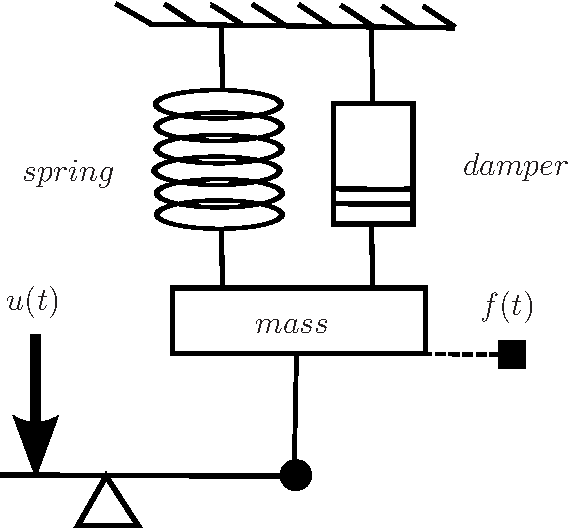
\includegraphics[width=0.5\columnwidth]{massSpringDamper}
\caption{A mass-spring-damper system to illustrate a latent force model with ordinary differential equations.}
\label{mass:spring:damper:figure}
\end{figure}

Our first illustrative example corresponds to the second order differential equation model described in equation \eqref{eq:sde0} with no control $c(t) = 0$. Figure~\ref{mass:spring:damper:figure} shows a mass-spring-damper system being forced by a latent function $u(t)$, which an example of a physical system that with such a model. The output $f(t)$ is also shown in the figure and represents the position of the body with a particular reference. For this model, we can compute the covariance function for $k_{f,f}(t,t')$ in equation \eqref{eq:fcov} using the following Green's function 
\begin{align}\label{Greens:ODE:2}
h(t-s) & = \frac{1}{\omega}\exp(-\alpha(t-s))\sin(\omega(t-s)),
\end{align} 
where $\omega = \sqrt{4\gamma - \lambda^2}/2$, and $\alpha =
\lambda/2$. 
If the covariance function $k(t-t')$ for the latent process $u(t)$  is a squared exponential (SE) covariance of the form 
\begin{align*}
k(t -t') = \sigma_t^2\exp\Bigg[-\frac{(t-t')^2}{\ell^2_t}\Bigg],
\end{align*}
it is possible to obtain closed-form solutions for $k_{f,f'}(t,t')$ and $k_{f,u}$ (see Eq. \eqref{eq:fucov}) \cite{Alvarez+Luengo+Lawrence:2009}.
 
We assume that the input source $u(t)$ is given as
\begin{align*}
u(t) = \sin(0.73t - 0.64) + \sin(0.29t- 0.64),
\end{align*}
where $t\in [0,50]$. The dashed line in Figure \ref{ode2:source:subfig:mlgp}  shows the input $u(t)$ computed for
$N=5000$ points equally distributed in the input domain. 

Parameters for the ODE are $\lambda = 0.1$, and $\gamma = 1$. The output function $f(t)$ obtained by solving the
differential equation is shown in Figure \ref{ode2:output:subfig:mlgp} as a dashed line. 
We uniformly choose $n=500$ time points $\{t_k\}_{k=1}^n$ within the interval $t\in [0,50]$, together with their
corresponding function evaluations $\{f_k\}_{k=1}^n$, as part of the training data. For the training points, we add Gaussian noise
$\epsilon_k$ with zero mean and variance equal to $0.09$, to get
measurements $\{y_k\}_{k=1}^n$. We assume that the parameters
$\lambda$, $\gamma$, and the variance for $\epsilon_k$ are known, and
only estimate the parameters $\sigma_t^2$,
and $\ell^2_t$ of the kernel function $k(t-t')$. The estimates were obtained by maximizing the log marginal likelihood by using the conjugate gradient method \cite{Rasmussen+Williams:2006}.

\begin{figure}[!ht]
\centering
       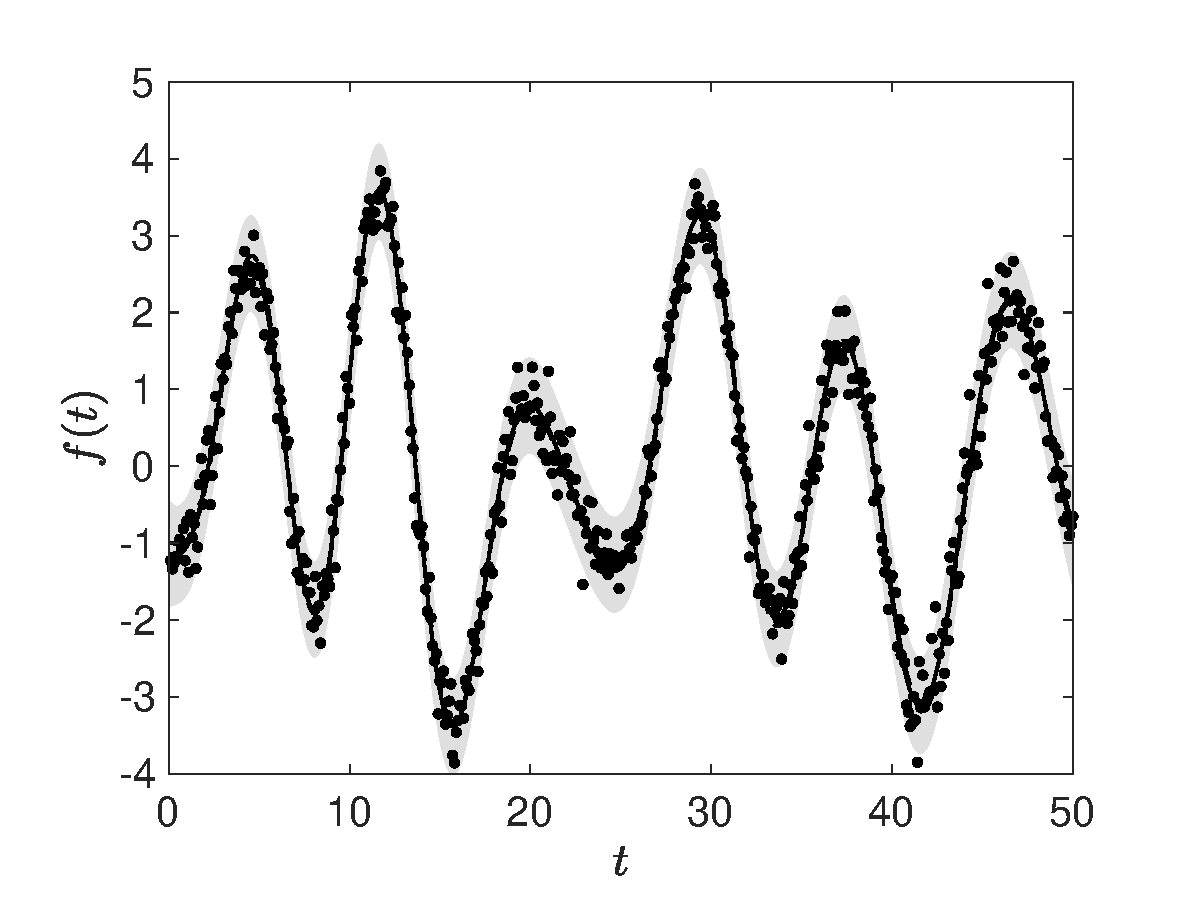
\includegraphics[width=0.7\columnwidth]{toyODE2output}
\caption{ODE output $f(t)$ and measurements $\{y_k\}_{k=1}^n$. The dashed line is the ground truth output $f(t)$
   obtained by solving the ODE, and the dots
   represent the noisy measurements $\{y_k\}_{k=1}^n$. The solid line is the predictive mean $f(t_*)$, and the grey
   region represents the predictive uncertainty, two standard deviations away from the mean prediction.\label{ode2:output:subfig:mlgp}}
\end{figure}

\begin{figure}[!ht]
\centering
       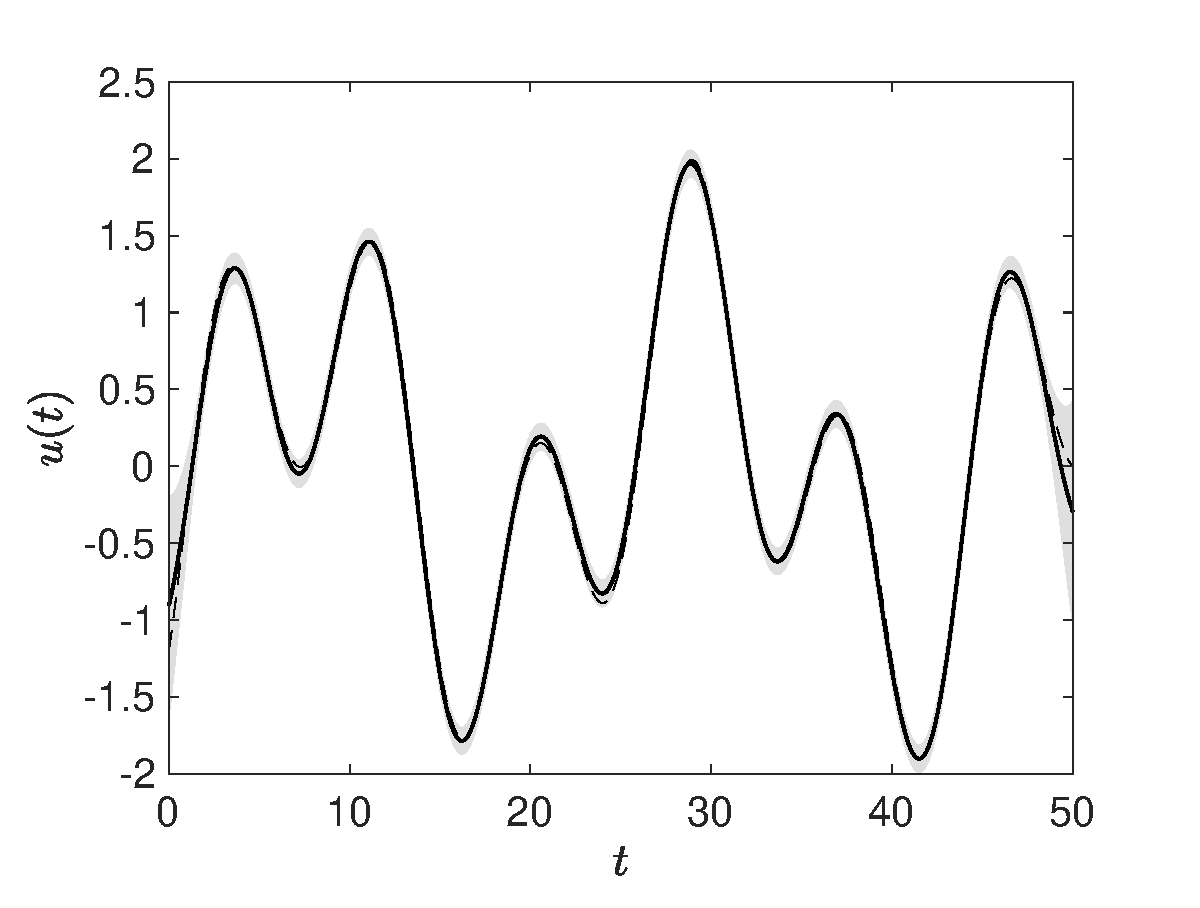
\includegraphics[width=0.7\columnwidth]{toyODE2source}
\caption{Ground truth and predicted source $u(t)$. The dashed line is the ground truth source $u(t)$. The solid
     line is the mean posterior for  $u^*$, while the shaded region covers two standard deviation away from the mean.\label{ode2:source:subfig:mlgp}}
\end{figure}

Results of inference for the latent function $u(t)$ are shown in Figure \ref{ode2:source:subfig:mlgp}. The mean squared error (MSE) between the ground truth source $u(t)$, and the inferred mean source $u^*(t)$ is equal to $0.0036$. The MSE between the ground truth output $f(t)$ and the mean predicted output $f^*(t)$ evaluated at the test input points is $0.0040$. As can be seen in the figure, the estimate is very close to the truth and the error quantiles are realistic.

The results above were obtained by explicitly computing the modified covariance function corresponding to the LFM. However, the result of using the equivalent state-space representation is practically the same, except for the minor differences due to the Pad\'e approximation required for the SE covariance function. Hence we do not show the state-space result here (it would be visually indistinguishable).

\subsection{Controlled ODE Model}

To demonstrate the benefit of the state-space representation and the modeling of the force as GP we consider the model \eqref{eq:sde0} with linear closed loop optimal control design for $c(t)$. In the experiment the mass-spring-damper system was started at static position $f(0) = -1$ and the aim was to keep it at the origin while the unknown latent force is affecting it. In the experiment we use the latent force hyper-parameters that were estimated from the open loop system considered in the previous section. We assumed that we only get measurements of the position, but with a relatively small variance $\sigma^2 = 0.01^2$---this was assumed to emphasize the differences between the control designs.

We consider two ways of designing the controller which were discussed in Section~\ref{sec:controlled_basic}: using the assumed separability design based on putting $u(t) = 0$ and a controller which is designed by taking account the existence of the latent force as described in the same section. The results of using the basic linear quadratic regulator (LQR), that is, the certainty equivalent design, and the result of using the joint LFM control are shown in Figure~\ref{fig:cntl_spring}. It can be seen that the LFM controller is able to maintain the system much better near the origin than the basic controller.

\begin{figure}[!t]
\centering
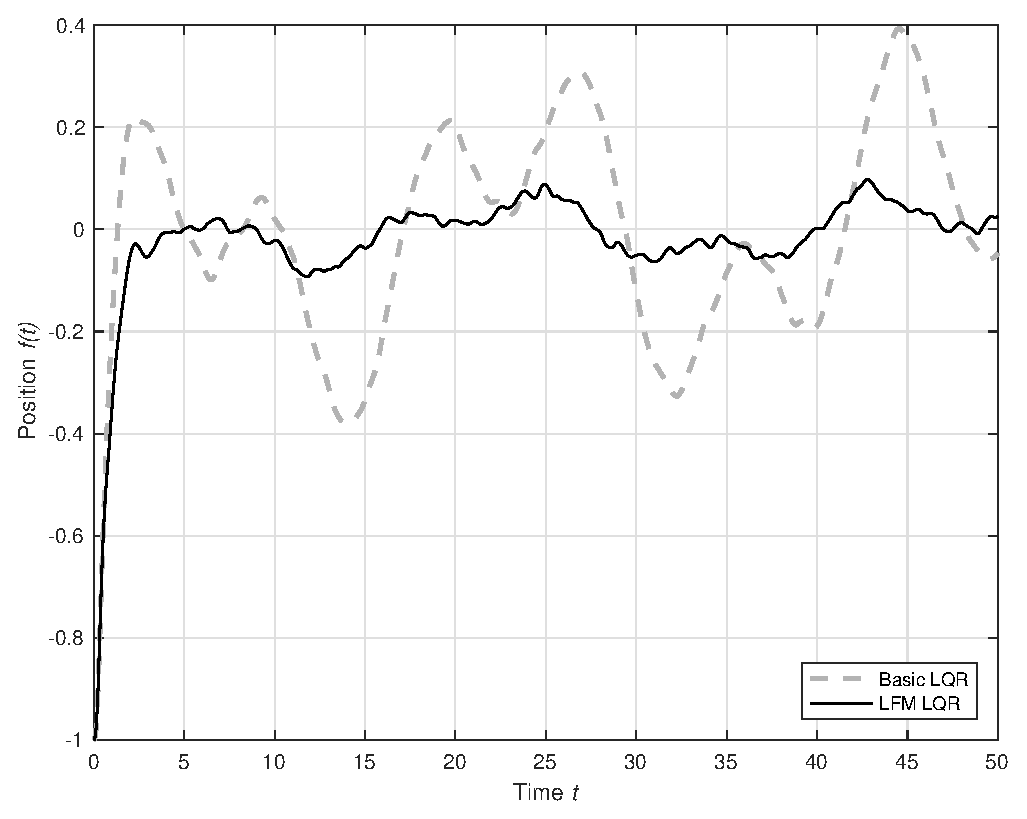
\includegraphics[width=0.7\columnwidth]{cntl_spring}
\caption{Result of controlling the ODE model with Basic LQR and LFM LQR. It can be seen the that control designed for the full LFM outperforms the basic LQR significantly. The average position tracking error for the Basic LFM was approximately $14.9$ units whereas in the case of LFM LQR it was approximately $7.8$ units.}
\label{fig:cntl_spring}
\end{figure}

%To estimate the state from the measurements we used a Kalman filter designed for the full latent state. The estimate produced by the Kalman filter is shown in Figure~\ref{fig:cntl_force}. The estimate is from the LFM LQR experiment, but the estimates with both the controllers are very similar.

%\begin{figure}[!t]
%\centering
%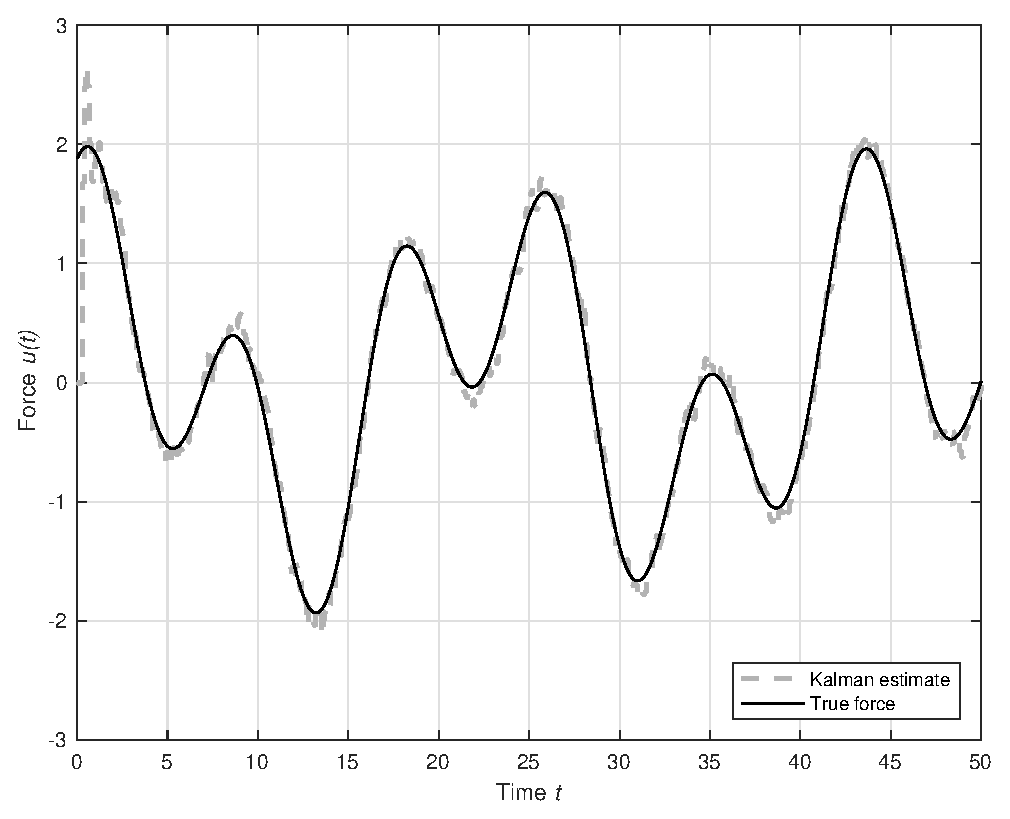
\includegraphics[width=0.8\columnwidth]{cntl_force}
%\caption{Kalman filter estimate of the latent force in the controlled ODE example. As expected, the estimate is worse in the beginning, but starts to follow the true force trajectory after the short initial transient.}
%\label{fig:cntl_force}
%\end{figure}


\subsection{Inference on Poisson equation}
%\simo{Mauricio: Finish the descriptions}


\begin{figure*}[!ht]
\centering
   \subfloat[Ground truth source function $u(x,y)$
   \label{pde:poisson:latent:gt}]{%
       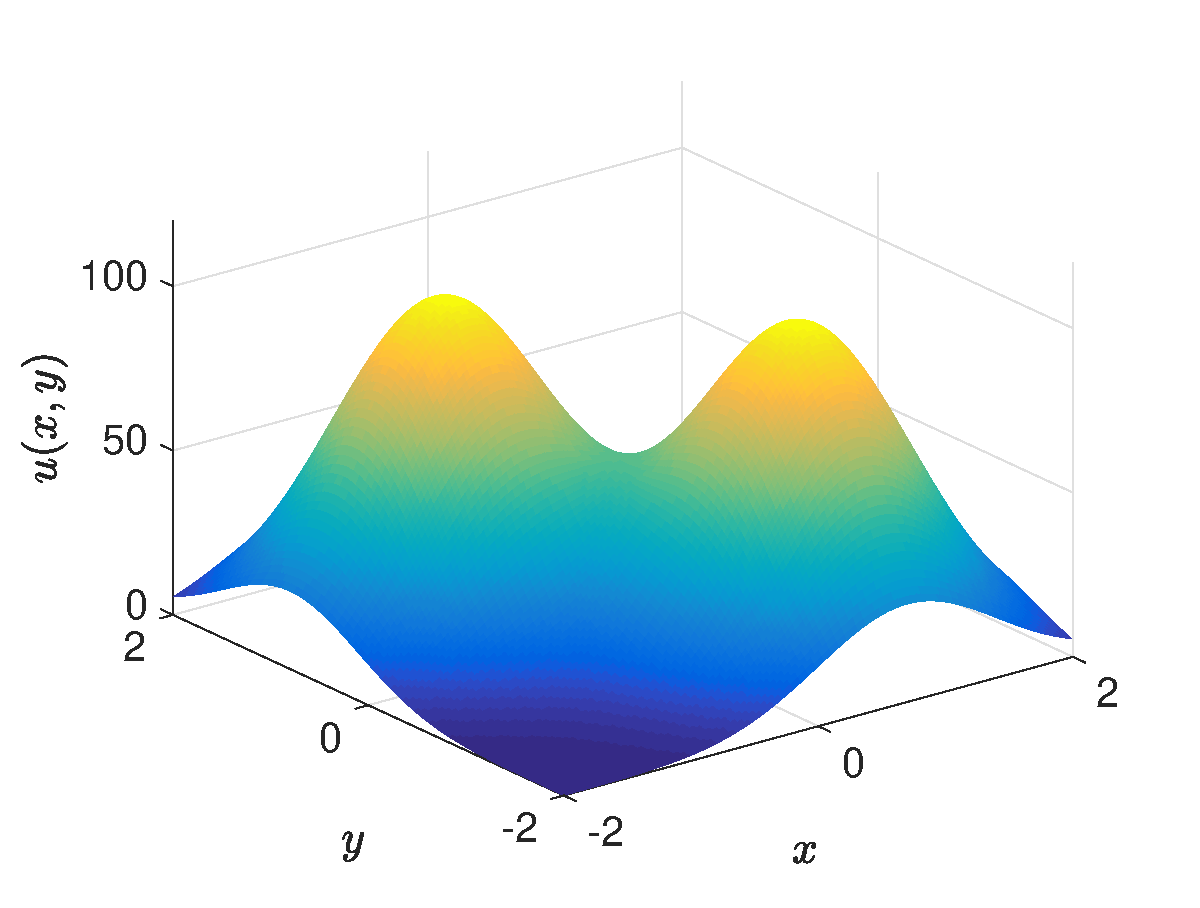
\includegraphics[width=0.33\textwidth]{toyPDElatentGT}
         }
     \subfloat[Contourns of the surface in Fig. \ref{pde:poisson:latent:gt} 
\label{pde:poisson:latent:gt:contour}]{%
       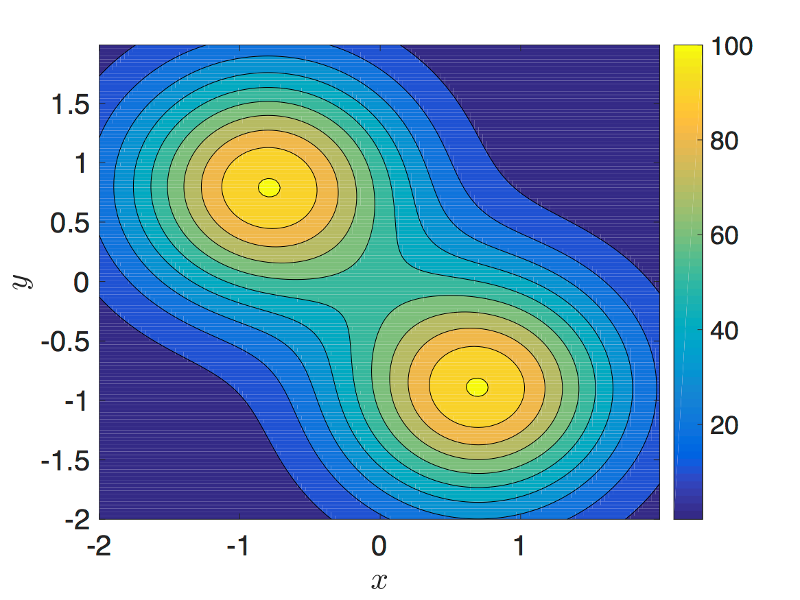
\includegraphics[width=0.3\textwidth]{toyPDElatentGTContourn}
     }
    \subfloat[Output function $f(x,y)$. 
    \label{pde:poisson:output:gt}]{%
       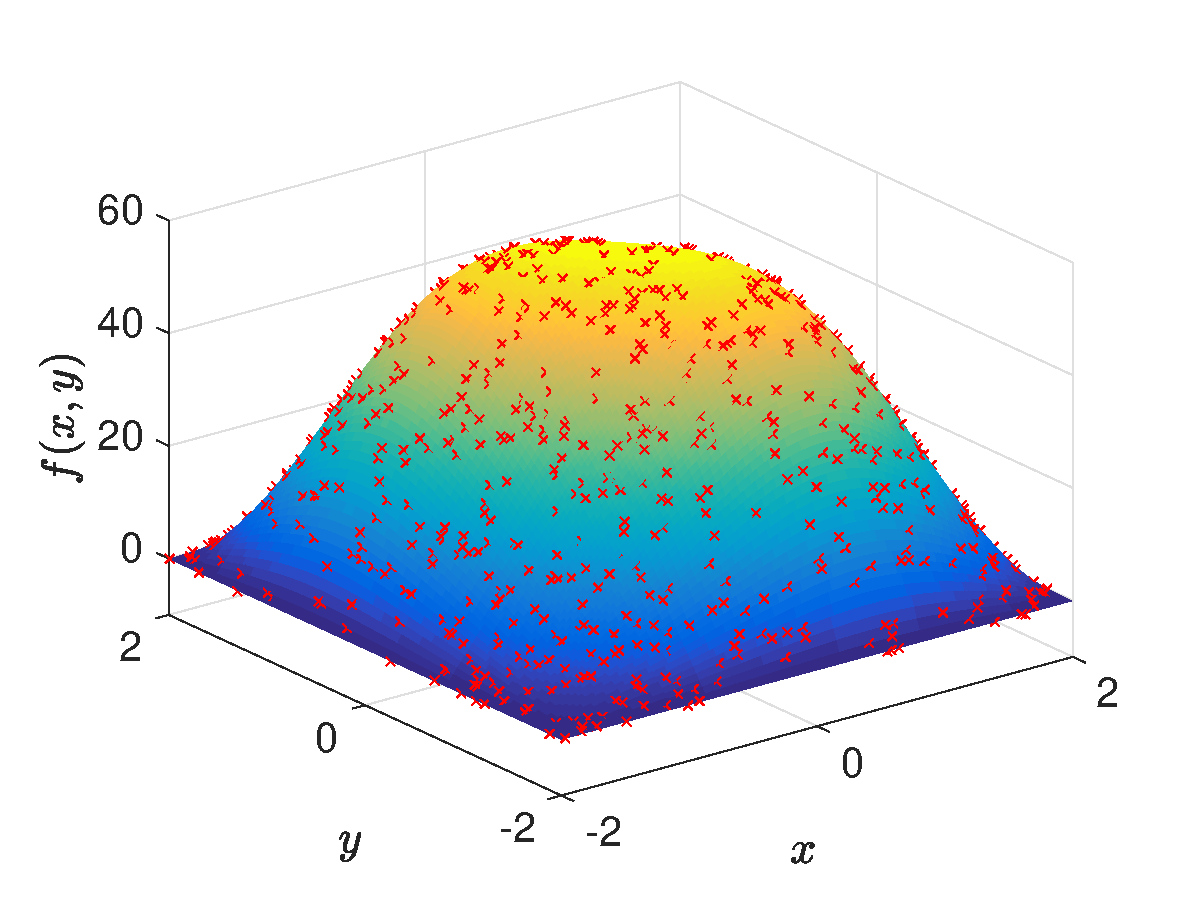
\includegraphics[width=0.33\textwidth]{toyPDEoutputGT}
     }\\
\subfloat[Mean prediction for $u^*(x,y)$.
\label{pde:poisson:latent:pr}]{%
       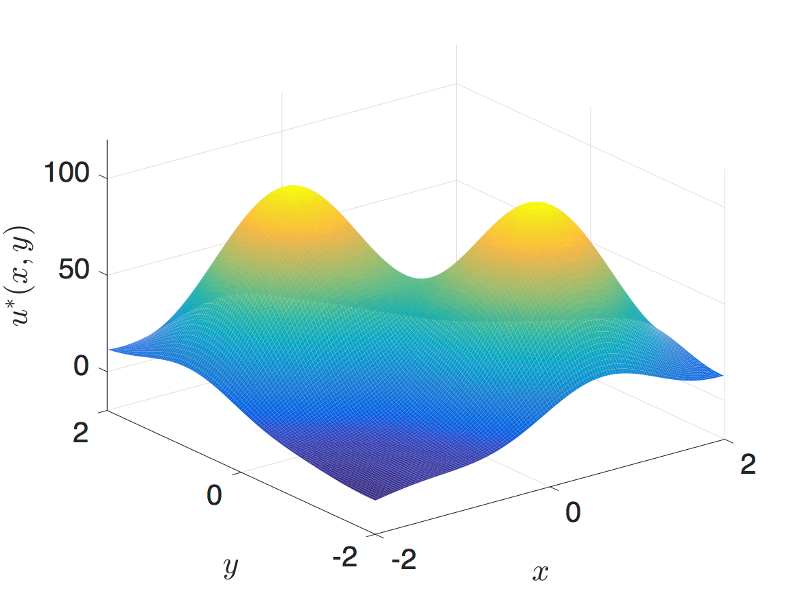
\includegraphics[width=0.33\textwidth]{toyPDElatentPR}
         }
     \subfloat[Contourns of the surface in Fig. \ref{pde:poisson:latent:pr} 
     \label{pde:poisson:latent:pr:contour}]{%
       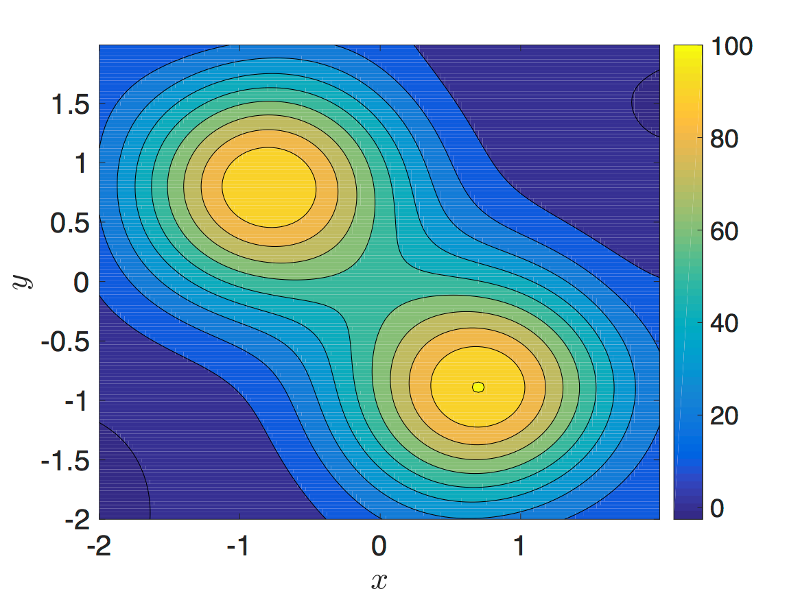
\includegraphics[width=0.3\textwidth]{toyPDElatentPRContourn}
     }
    \subfloat[Mean prediction for $f^*(x,y)$     
    \label{pde:poisson:output:pr}]{%
       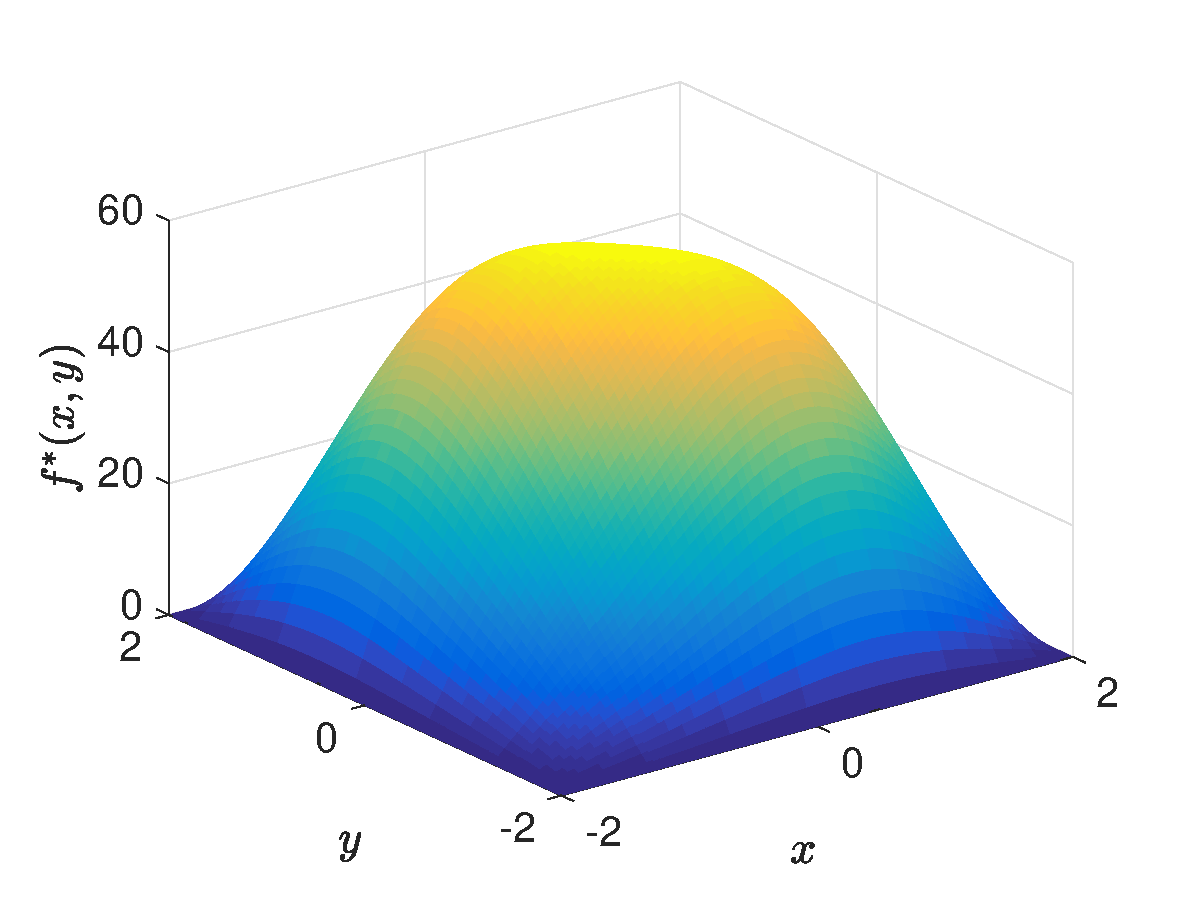
\includegraphics[width=0.33\textwidth]{toyPDEoutputPR}
     }

     \caption{The upper row shows the ground truth data for the 2D PDE Poisson example: the input source
       (Fig. \ref{pde:poisson:latent:gt}); contours of the ground truth input source
       \ref{pde:poisson:latent:gt:contour}; ground truth for the output function
       (Fig. \ref{pde:poisson:output:gt}). Noisy observations are shown as red crosses in
       Fig. \ref{pde:poisson:output:gt}. The lower row shows the predicted mean function
       $\mathbb{E}[u^*(x,y)|\mathbf{y}]$ (Fig. \ref{pde:poisson:latent:pr}); contours of the predicted mean function
       (Fig. \ref{pde:poisson:latent:pr:contour}); the predicted mean output $\mathbb{E}[f^*(x,y)|\mathbf{y}]$ 
      (Fig. \ref{pde:poisson:output:pr}). Noisy observations are again shown as red crosses in Fig. \ref{pde:poisson:output:pr}. 
     }
     \label{fig:dummy}
   \end{figure*}



In this example, we model the 2D Poisson equation where our aim is to infer the unknown input field $u(x,y)$ from noisy
observations $y_k$, as in Eq. \eqref{eq:sde0}. We assume that the source follows
a GP prior with an SE covariance. The input space consists of two space variables that we refer to as $x$
and $y$. The covariance function for the source is given as
\begin{align*}
k(x-x', y -y') = \exp\Bigg[-\frac{(x-x')^2}{\sigma^2_x}\Bigg]\exp\Bigg[-\frac{(y-y')^2}{\sigma^2_y}\Bigg],
\end{align*}
where $\sigma_x$, and $\sigma_y$ are the length-scales along the
spatial dimensions.

Assuming boundary conditions equal to zero, we can use the corresponding Green's function (see
\cite{Polyanin:Handbook02} for mathematical details) to compute covariance functions for the output
$k_{f,f}(x,y,x',y')$, and between the output and the latent source $k_{f,u}(x,y,x',y')$. We can then use GP regression
expressions to infer the posterior distribution $p(u^* \mid \mathbf{y})$.

In this example, the input field $u(x,y)$ is given by
\begin{align*}
u(x, y) & = 100\exp\left\{- \frac{\left[(x + 0.8)^2 + (y - 0.8)^2\right]}{s^2}\right\} \\
         & + 100\exp\left\{- \frac{\left[(x - 0.7)^2 + (y + 0.9)^2\right]}{s^2}\right\},
\end{align*}
where $s^2 = 1$.
Figure \ref{pde:poisson:latent:gt} shows a 3D description of the input source in the domain $[-2, 2]\times
[-2,2]$. Figure \ref{pde:poisson:latent:gt:contour} shows contours of the same input source. Figure
\ref{pde:poisson:output:gt} corresponds to the output function $f(t)$ obtained by solving the Poisson equation with an
input source given by the function in Figure \ref{pde:poisson:latent:gt}.



   The output function is made of $17,956$ observation points distributed in a grid of $134\times 134$ inputs uniformly
   organized in the input domain. From those observations, we randomly choose $n=1000$ spatial points with their
   corresponding function evaluations $\{f_k\}_{k=1}^n$ as part of the data used to estimate the parameters $\sigma_x^2$
   and $\sigma_y^2$. Furthermore, we add Gaussian noise with variance $0.01$ to the function evaluations, and obtain the
   noisy observations $\{y_k\}_{k=1}^n$. Figure \ref{pde:poisson:output:gt} shows the noisy observations as red crosses.
   For obtaining estimates of $\sigma_x^2$ and $\sigma_y^2$, we maximize the marginal log-likelihood function with
   respect to the parameters.

Figure \ref{pde:poisson:latent:pr} shows the mean prediction of the distribution $p(u^* \mid \mathbf{y})$. Figure
\ref{pde:poisson:latent:pr:contour} shows contours for the estimated mean function. We notice that the mean predictive
function $\mathbb{E}[u^*(x,y) \mid \mathbf{y}]$ is qualitatively similar to the ground truth function $u(x,y)$. Figure
\ref{pde:poisson:output:pr} shows the mean of the predictive distribution $p(f^*(x,y) \mid \mathbf{y})$. We note the
similarity between the ground truth in Figure \ref{pde:poisson:output:gt} and the mean prediction in Figure
\ref{pde:poisson:output:pr}.  Furthermore, the MSE between the ground truth source $u(x,y)$, and the inferred mean source $u^*(x,y)$
is equal to $0.5153$. The MSE between the ground truth output $f(x,y)$ and the mean predicted output $f^*(x,y)$
evaluated at the test input points is $8.3354\times 10^{-4}$.

% \simo{Mauricio writes the Poisson 2D example here and we use both series expansion and closed-form methods here. We leave the state-space version out because, as discussed a few sections ago, it is not at all suitable in this case.}

%\begin{equation}
%\begin{split}
%    \frac{\partial\mathbf{u}(\mathbf{x},t)}{\partial t} &= \mathbf{\mathcal{A}}_u \, \mathbf{u}(\mathbf{x},t)
%  + \mathbf{B}_u \, w(\mathbf{x},t) \\
%  \frac{\partial \mathbf{f}(\mathbf{x},t)}{\partial t} &= 
%       \begin{pmatrix} 
%        0 & 1 \\ 
%        \frac{\partial^2}{\partial x^2}
%        & -2 \sqrt{-\frac{\partial^2}{\partial x^2}} 
%      \end{pmatrix}\mathbf{u}(\mathbf{x},t)
%      + \begin{pmatrix} 0 \\ 1 \end{pmatrix} \mathbf{C}_u \, \mathbf{u}(\mathbf{x},t), \\
%      f(\mathbf{x},t) &= \begin{pmatrix} 1 & 0 \end{pmatrix} \, \mathbf{f}(\mathbf{x},t),
%\end{split}
%\end{equation}
%

% \subsection{LQ Control of ODE LFMs}

% \simo{Simo: State-space control of string model with comparison to non-LFM control.}

\subsection{Controlled heat equation}

In this experiment we consider a controlled heat equation of the form
%
\begin{equation}
  \frac{\partial f(\mathbf{x},t)}{\partial t} = - \lambda f(\mathbf{x},t) + D \, \nabla^2 f(\mathbf{x},t)
  + u(\mathbf{x},t) + c(\mathbf{x},t),
\end{equation}
%
where $u(\mathbf{x},t)$ is an unknown latent force, $c(\mathbf{x},t)$ is the control signal, $\mathbf{x} \in \mathbb{R}^2$, and $\lambda,D > 0$ are positive constants. Figure \ref{cartoon:heatpde} is a cartoon representation of the simulated scenario which is a heat source moving across a 2D spatial field. The field is measured at a discrete grid and the measurements are corrupted by Gaussian noise. In the simulation, the latent force $u(\mathbf{x},t)$ is the heat generated by the moving source and the aim is to reconstruct $f$ and $u$ from noisy observations as well as design an optimal control signal $c(\mathbf{x},t)$, which aims to regulate the temperature $f(\mathbf{x},t)$ to zero.

\begin{figure}[!t]
\centering
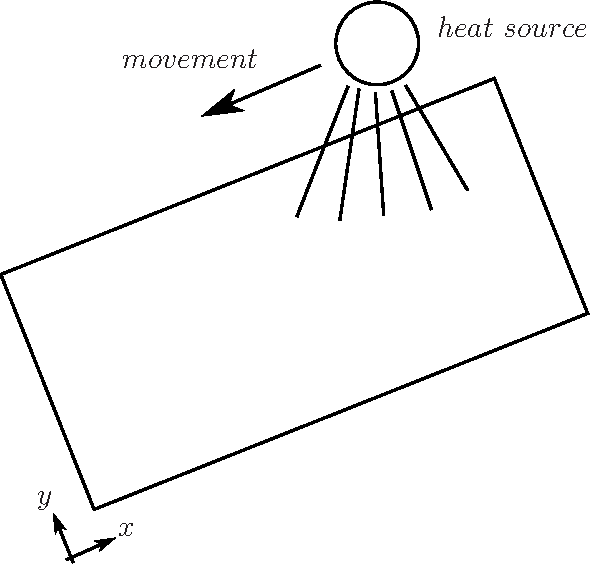
\includegraphics[width=0.5\columnwidth]{heatpde}
\caption{A cartoon representation of a heat source moving across a 2D spatial field.}
\label{cartoon:heatpde}
\end{figure}

In the simulation, we used the parameters $\lambda = 0.2$ and $D = 0.001$ and the heat source was moving for 10 seconds from top-right to bottom-left direction and then it was turned off. The temperature then increases at the application point and when the heat source moves away, the position starts cooling down. Figures~\ref{fig:heat_open_x} and \ref{fig:heat_open_u} show the temperature field and the heat source at time $t = 6.9$ when no control is applied. 

\begin{figure}[!t]
\centering
   \subfloat[Temperature field $f(\mathbf{x},t)$
   \label{fig:heat_open_x}]{%
       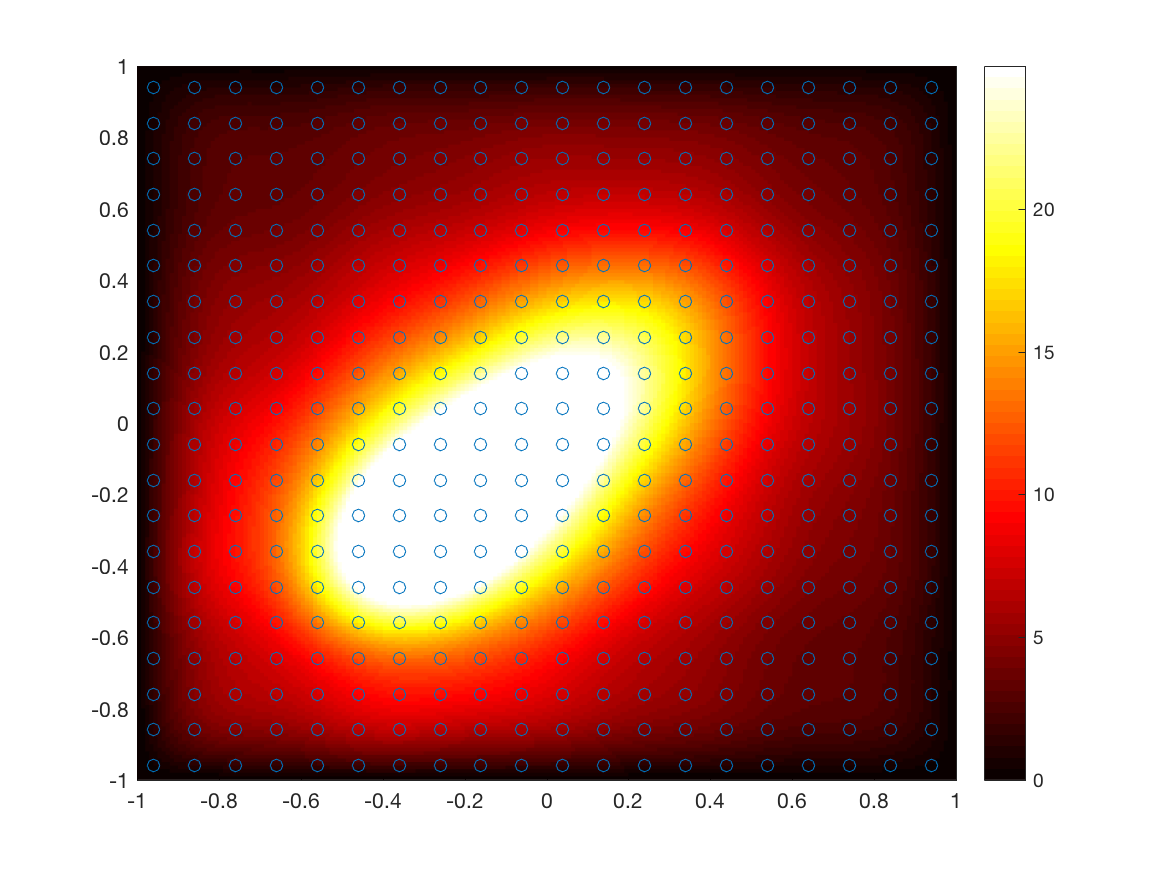
\includegraphics[width=0.49\columnwidth]{heat_open_x}
         }
   \subfloat[Source field $u(\mathbf{x},t)$
   \label{fig:heat_open_u}]{%
       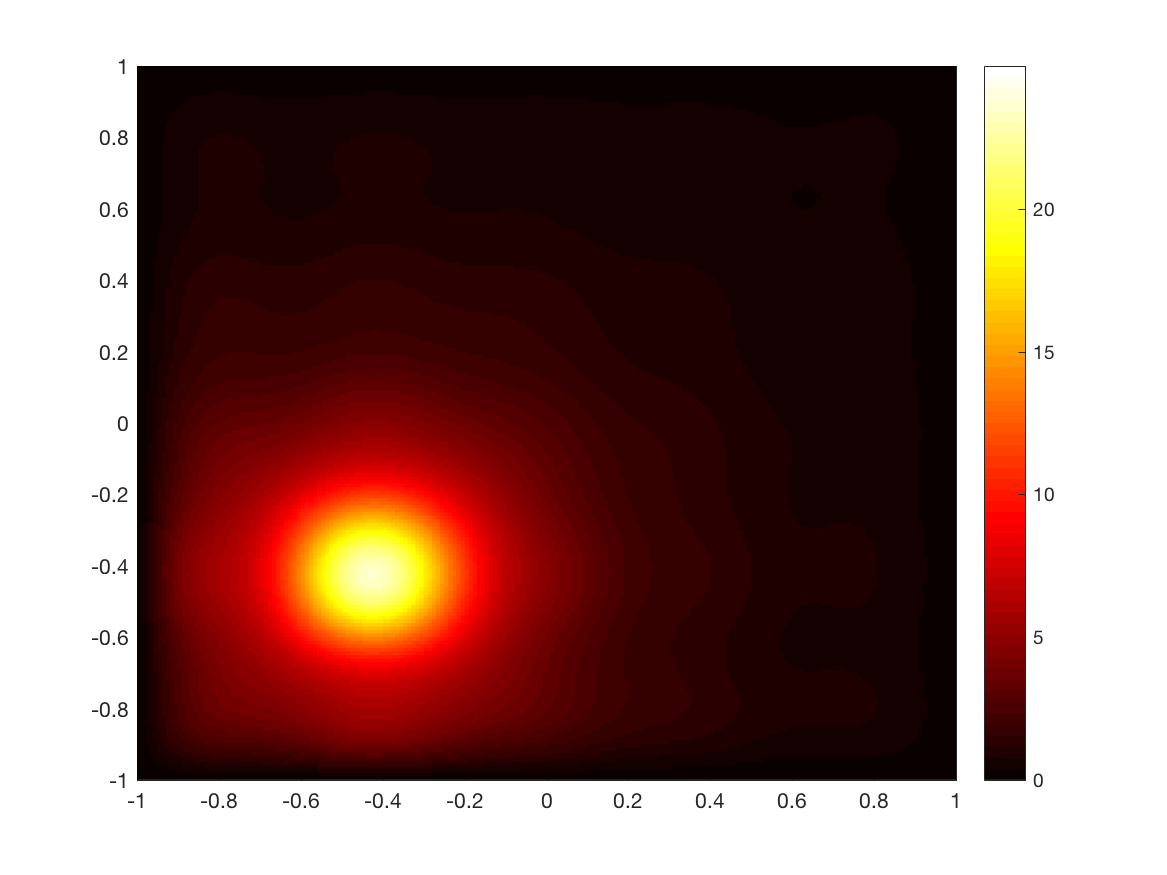
\includegraphics[width=0.49\columnwidth]{heat_open_u}
         }
\caption{The temperature function $f(\mathbf{x},t)$ and the source function $u(\mathbf{x},t)$ at time $t = 6.9$. The small circles mark the positions of the measurements.}
\end{figure}

We then formed a Fourier-basis approximation to the PDE (with $100$ basis functions) and designed two controllers for it---one using an assumed separability design ("Basic LQR") and one by taking the latent force into account ("LFM LQR"). We used SE covariance functions for the latent force model in both time and space directions. A Kalman filter was used to estimate the physical system and latent force states from temperature measurements with low variance ($\sigma^2 = 0.01^2$) and the controller was applied using the estimate.

\begin{figure}[!t]
\centering
   \subfloat[Field $f(\mathbf{x},t)$ with Basic LQR 
   \label{fig:heat_lq_x}]{%
       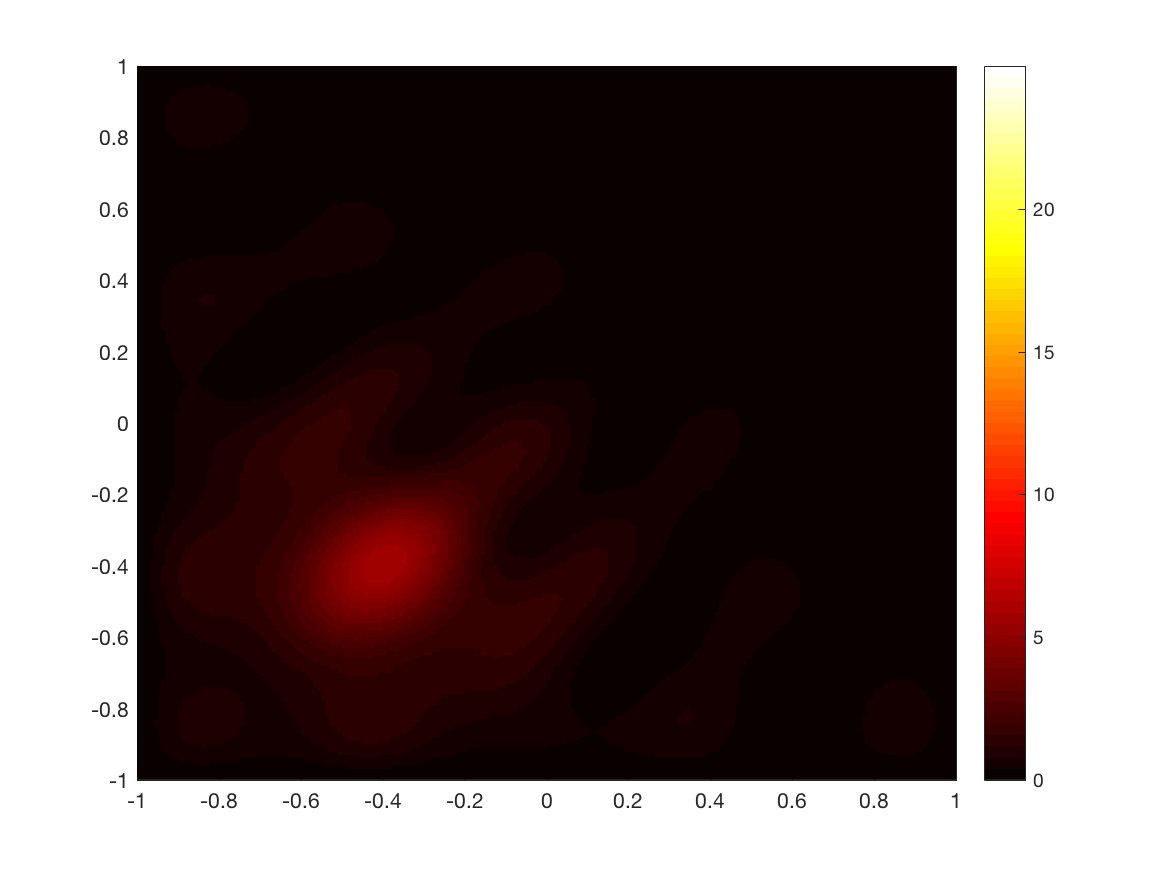
\includegraphics[width=0.49\columnwidth]{heat_lq_x}
         }
   \subfloat[Field $f(\mathbf{x},t)$ with LFM LQR
   \label{fig:heat_lfm_lq_x}]{%
       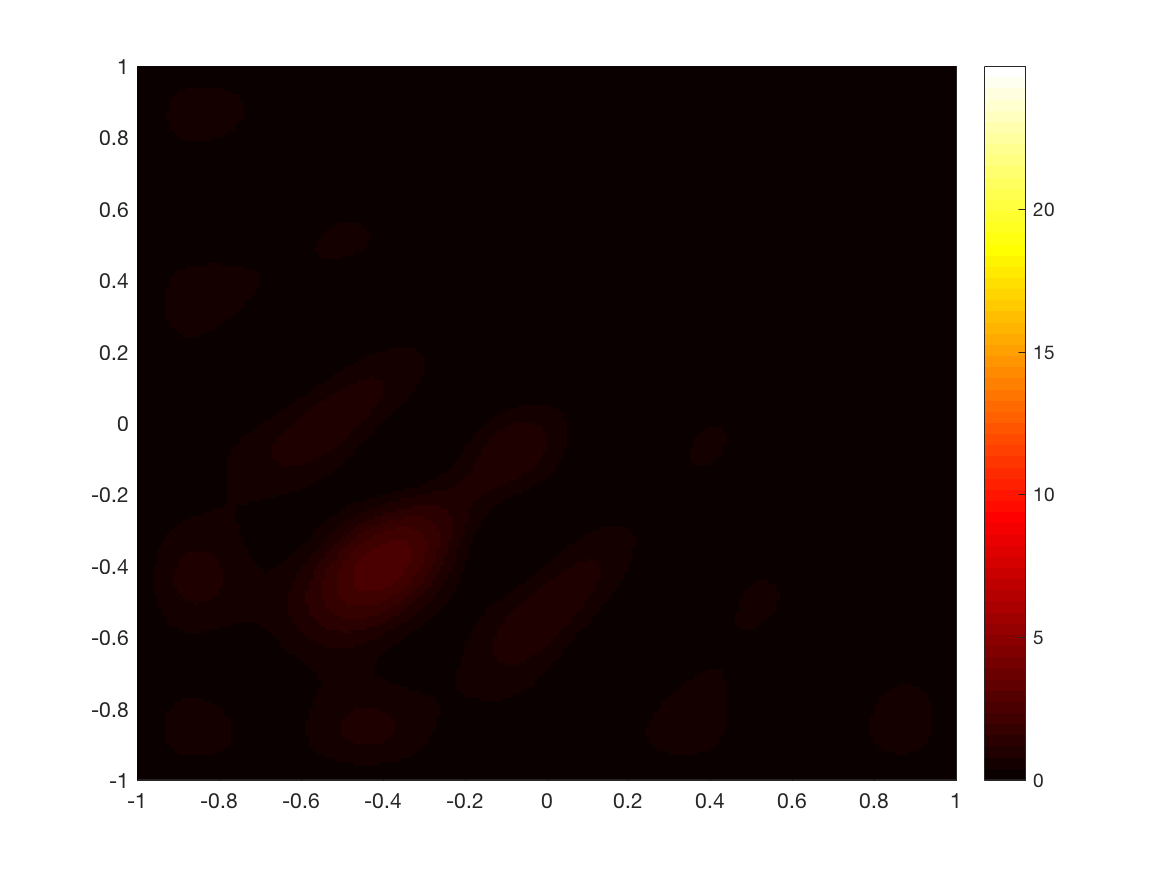
\includegraphics[width=0.49\columnwidth]{heat_lfm_lq_x}
         }
  \\
   \subfloat[Maximum temperatures
   \label{fig:heat_maxtemp}]{%
       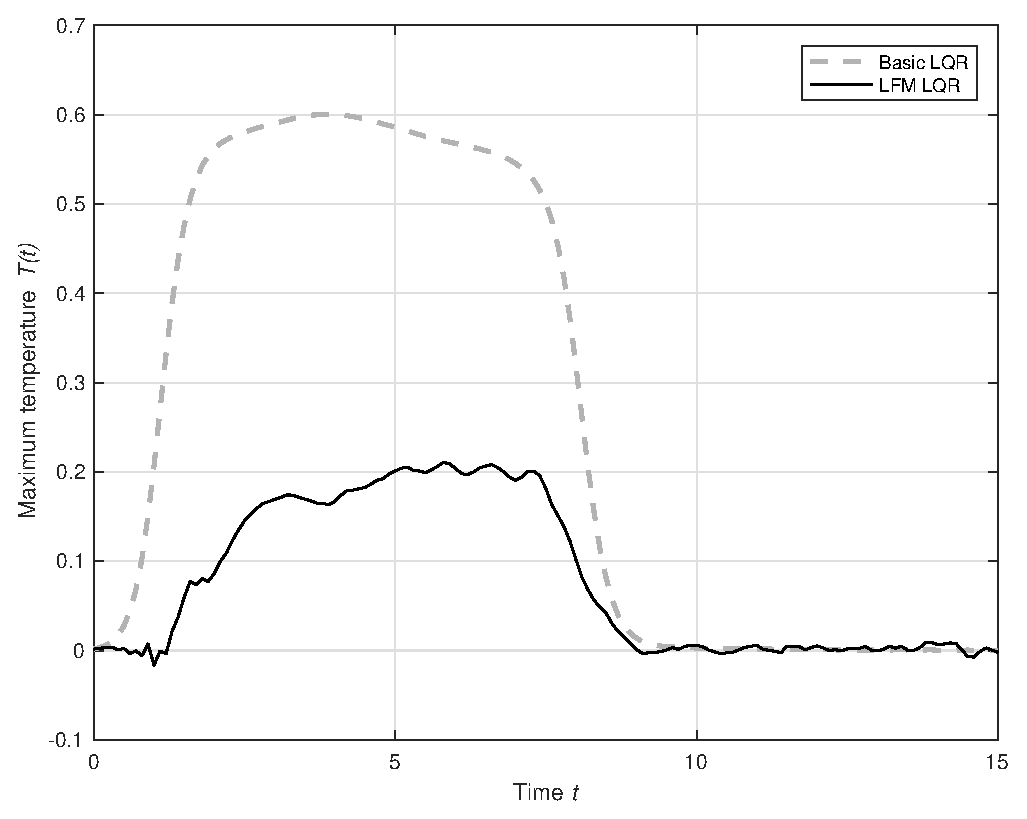
\includegraphics[width=0.49\columnwidth]{heat_maxtemp}
         }
   \subfloat[LFM control signal
   \label{fig:heat_lfm_lq_c}]{%
       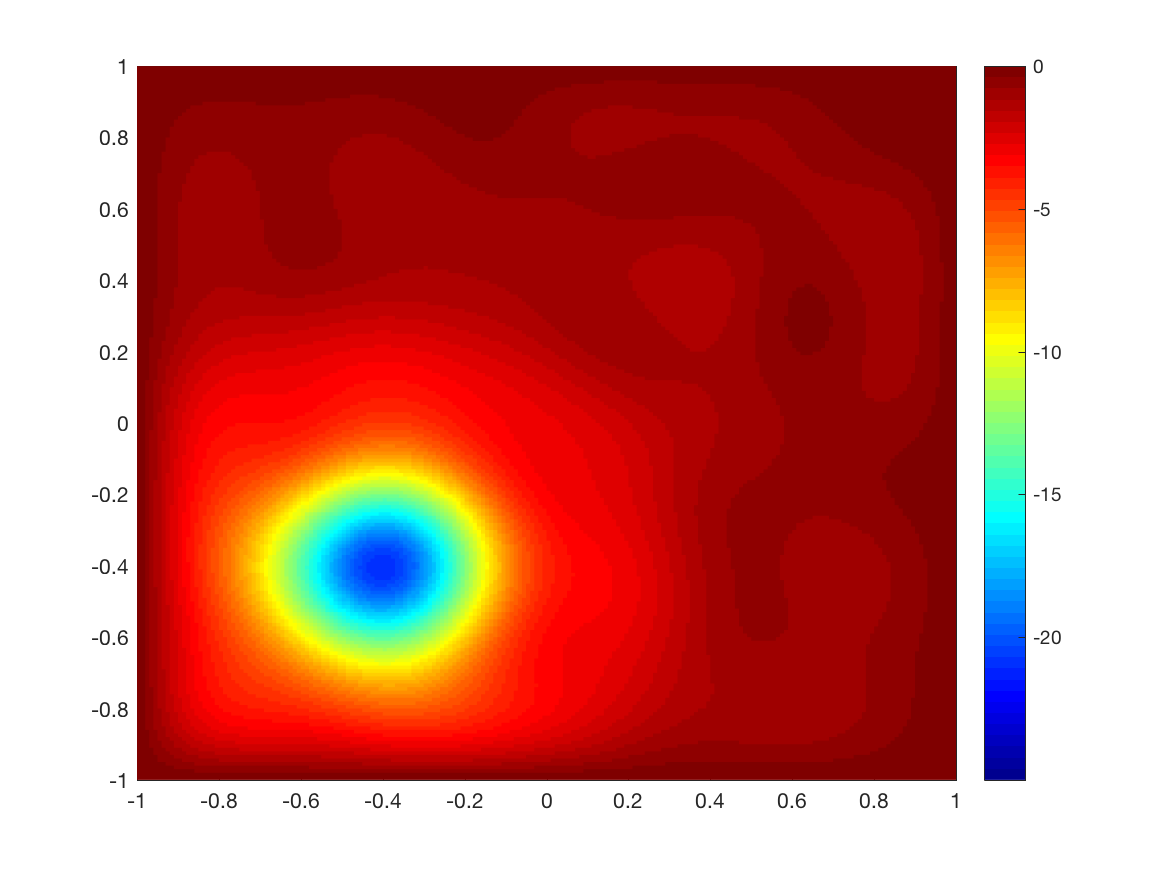
\includegraphics[width=0.49\columnwidth]{heat_lfm_lq_c}
         }
\caption{The results of using Basic LQR and LFM LQR controllers to regulate the temperature field to zero. It can be seen from Figures~\ref{fig:heat_lq_x},  \ref{fig:heat_lfm_lq_x}, and \ref{fig:heat_maxtemp} that LFM LQR is able to keep the temperature closer to zero than Basic LQR. Figure~\ref{fig:heat_lfm_lq_c} shows an example control signal which can be see to effectively cancel out the latent force model part as one would expect.}
\end{figure}

Figures~\ref{fig:heat_lq_x} -- \ref{fig:heat_lfm_lq_c} show the results when the controllers were used. It can be seen that the LFM LQR provides a significantly smaller tracking error. 



%\subsection{\simo{\st{A Periodic Model}}}

%\simo{Probably leave this out}

\section{Conclusions}
In this paper we have presented a latent force model (LFM) framework for learning and control in hybrid systems which are combinations of first-principles (physical) models and non-parametric Gaussian process models as their inputs. We have presented both covariance function based inference methods and state-space based inference methods for the models as well as analyzed the detectability and observability properties of LFMs. Additionally, we have extended the methodology to allow for stochastic control of the (state-space) LFMs. Although the full models are uncontrollable, they are output controllable with respect to the physical model part which is enough for practical implementation of the controllers.


% if have a single appendix:
%\appendix[Proof of the Zonklar Equations]
% or
%\appendix  % for no appendix heading
% do not use \section anymore after \appendix, only \section*
% is possibly needed

% use appendices with more than one appendix
% then use \section to start each appendix
% you must declare a \section before using any
% \subsection or using \label (\appendices by itself
% starts a section numbered zero.)
%


%\appendices
%\section{Proof of the First Zonklar Equation}
%Appendix one text goes here.

% you can choose not to have a title for an appendix
% if you want by leaving the argument blank
%\section{}
%Appendix two text goes here.


% use section* for acknowledgment
%\section*{Acknowledgment}


%The authors would like to thank Academy of Finland for funding.


% Can use something like this to put references on a page
% by themselves when using endfloat and the captionsoff option.
\ifCLASSOPTIONcaptionsoff
  \newpage
\fi



% trigger a \newpage just before the given reference
% number - used to balance the columns on the last page
% adjust value as needed - may need to be readjusted if
% the document is modified later
%\IEEEtriggeratref{8}
% The "triggered" command can be changed if desired:
%\IEEEtriggercmd{\enlargethispage{-5in}}

% references section

% can use a bibliography generated by BibTeX as a .bbl file
% BibTeX documentation can be easily obtained at:
% http://mirror.ctan.org/biblio/bibtex/contrib/doc/
% The IEEEtran BibTeX style support page is at:
% http://www.michaelshell.org/tex/ieeetran/bibtex/
\bibliographystyle{IEEEtran}
% argument is your BibTeX string definitions and bibliography database(s)
\bibliography{reviewlfm}
%
% <OR> manually copy in the resultant .bbl file
% set second argument of \begin to the number of references
% (used to reserve space for the reference number labels box)
%\begin{thebibliography}{1}

%\bibitem{IEEEhowto:kopka}
%H.~Kopka and P.~W. Daly, \emph{A Guide to \LaTeX}, 3rd~ed.\hskip 1em plus
 % 0.5em minus 0.4em\relax Harlow, England: Addison-Wesley, 1999.
%
%\end{thebibliography}

% biography section
% 
% If you have an EPS/PDF photo (graphicx package needed) extra braces are
% needed around the contents of the optional argument to biography to prevent
% the LaTeX parser from getting confused when it sees the complicated
% \includegraphics command within an optional argument. (You could create
% your own custom macro containing the \includegraphics command to make things
% simpler here.)
%\begin{IEEEbiography}[{\includegraphics[width=1in,height=1.25in,clip,keepaspectratio]{mshell}}]{Michael Shell}
% or if you just want to reserve a space for a photo:

\begin{IEEEbiography}{Michael Shell}
Biography text here.
\end{IEEEbiography}

% if you will not have a photo at all:
\begin{IEEEbiographynophoto}{John Doe}
Biography text here.
\end{IEEEbiographynophoto}

% insert where needed to balance the two columns on the last page with
% biographies
%\newpage

\begin{IEEEbiographynophoto}{Jane Doe}
Biography text here.
\end{IEEEbiographynophoto}

% You can push biographies down or up by placing
% a \vfill before or after them. The appropriate
% use of \vfill depends on what kind of text is
% on the last page and whether or not the columns
% are being equalized.

%\vfill

% Can be used to pull up biographies so that the bottom of the last one
% is flush with the other column.
%\enlargethispage{-5in}



% that's all folks
\end{document}


